% Options for packages loaded elsewhere
\PassOptionsToPackage{unicode}{hyperref}
\PassOptionsToPackage{hyphens}{url}
%
\documentclass[
  ignorenonframetext,
]{beamer}
\usepackage{pgfpages}
\setbeamertemplate{caption}[numbered]
\setbeamertemplate{caption label separator}{: }
\setbeamercolor{caption name}{fg=normal text.fg}
\beamertemplatenavigationsymbolsempty
% Prevent slide breaks in the middle of a paragraph
\widowpenalties 1 10000
\raggedbottom
\setbeamertemplate{part page}{
  \centering
  \begin{beamercolorbox}[sep=16pt,center]{part title}
    \usebeamerfont{part title}\insertpart\par
  \end{beamercolorbox}
}
\setbeamertemplate{section page}{
  \centering
  \begin{beamercolorbox}[sep=12pt,center]{part title}
    \usebeamerfont{section title}\insertsection\par
  \end{beamercolorbox}
}
\setbeamertemplate{subsection page}{
  \centering
  \begin{beamercolorbox}[sep=8pt,center]{part title}
    \usebeamerfont{subsection title}\insertsubsection\par
  \end{beamercolorbox}
}
\AtBeginPart{
  \frame{\partpage}
}
\AtBeginSection{
  \ifbibliography
  \else
    \frame{\sectionpage}
  \fi
}
\AtBeginSubsection{
  \frame{\subsectionpage}
}
<<<<<<< Updated upstream
\usepackage{lmodern}
\usepackage{amssymb,amsmath}
\usepackage{ifxetex,ifluatex}
\ifnum 0\ifxetex 1\fi\ifluatex 1\fi=0 % if pdftex
=======
\usepackage{amsmath,amssymb}
\usepackage{iftex}
\ifPDFTeX
>>>>>>> Stashed changes
  \usepackage[T1]{fontenc}
  \usepackage[utf8]{inputenc}
  \usepackage{textcomp} % provide euro and other symbols
\else % if luatex or xetex
  \usepackage{unicode-math}
  \defaultfontfeatures{Scale=MatchLowercase}
  \defaultfontfeatures[\rmfamily]{Ligatures=TeX,Scale=1}
\fi
<<<<<<< Updated upstream
\usetheme[]{default}
\usefonttheme{professionalfonts}
=======
\usepackage{lmodern}
\usetheme[]{default}
\usefonttheme{professionalfonts}
\ifPDFTeX\else
  % xetex/luatex font selection
\fi
>>>>>>> Stashed changes
% Use upquote if available, for straight quotes in verbatim environments
\IfFileExists{upquote.sty}{\usepackage{upquote}}{}
\IfFileExists{microtype.sty}{% use microtype if available
  \usepackage[]{microtype}
  \UseMicrotypeSet[protrusion]{basicmath} % disable protrusion for tt fonts
}{}
\makeatletter
\@ifundefined{KOMAClassName}{% if non-KOMA class
  \IfFileExists{parskip.sty}{%
    \usepackage{parskip}
  }{% else
    \setlength{\parindent}{0pt}
    \setlength{\parskip}{6pt plus 2pt minus 1pt}}
}{% if KOMA class
  \KOMAoptions{parskip=half}}
\makeatother
\usepackage{xcolor}
<<<<<<< Updated upstream
\IfFileExists{xurl.sty}{\usepackage{xurl}}{} % add URL line breaks if available
\IfFileExists{bookmark.sty}{\usepackage{bookmark}}{\usepackage{hyperref}}
\hypersetup{
  pdftitle={Inferencia causal},
  hidelinks,
  pdfcreator={LaTeX via pandoc}}
\urlstyle{same} % disable monospaced font for URLs
=======
>>>>>>> Stashed changes
\newif\ifbibliography
\usepackage{graphicx}
\makeatletter
\def\maxwidth{\ifdim\Gin@nat@width>\linewidth\linewidth\else\Gin@nat@width\fi}
\def\maxheight{\ifdim\Gin@nat@height>\textheight\textheight\else\Gin@nat@height\fi}
\makeatother
% Scale images if necessary, so that they will not overflow the page
% margins by default, and it is still possible to overwrite the defaults
% using explicit options in \includegraphics[width, height, ...]{}
\setkeys{Gin}{width=\maxwidth,height=\maxheight,keepaspectratio}
% Set default figure placement to htbp
\makeatletter
\def\fps@figure{htbp}
\makeatother
\setlength{\emergencystretch}{3em} % prevent overfull lines
\providecommand{\tightlist}{%
  \setlength{\itemsep}{0pt}\setlength{\parskip}{0pt}}
\setcounter{secnumdepth}{-\maxdimen} % remove section numbering
\usepackage{fancyhdr}
\usepackage{lastpage}
\setbeamertemplate{navigation symbols}{}
\setbeamertemplate{footline}[page number]
\pagenumbering{arabic}
% \usepackage[mathbf,mathcal]{euler}


\title{Inferencia causal}
\author{Diseño e implementación de experimentos en ciencias sociales\\
\emph{Departamento de Economía (UdelaR)}}
\date{}

\begin{document}
\frame{\titlepage}

\begin{frame}{Tema 1. Inferencia causal}
\protect\hypertarget{tema-1.-inferencia-causal}{}
\begin{itemize}
\tightlist
\item
  El modelo de causalidad Neyman--Rubin
\item
  Experimentos aleatorizados y validez
\item
  Asignación aleatoria simple
\item
  Estimandos (ATE, ITT, CACE, SATE, PATE, ATT, CATE, mediación)
\end{itemize}
\end{frame}

\begin{frame}{Lecturas}
\protect\hypertarget{lecturas}{}
\begin{itemize}
\item
  Gerber, Alan S., and Donald P. Green. 2012. \emph{Field Experiments:
  Design, Analysis, and Interpretation.} New York: W.W. Norton. (FEDAI).
  capítulos 1-2.
\item
  Imbens, G. W., \& Rubin, D. B. (2015). Causal inference in statistics,
  social, and biomedical sciences. Cambridge University Press. (CISSBS),
  capítulos 1-2.
\item
  \href{https://egap.org/resource/10-types-of-treatment-effect-you-should-know-about/}{10
  Types of Treatment Effect You Should Know About}
\item
  Aronow, P. M. and Samii, C. (2016). ``Does regression produce
  representative estimates of causal effects?'' \emph{American Journal
  of Political Science}, 60(1):250--267
\item
  Barabas, J. and Jerit, J. (2010). ``Are survey experiments externally
  valid?'' \emph{American Political Science Review}, 104(2):226--242
\end{itemize}
\end{frame}

\hypertarget{causalidad}{%
\section{Causalidad}\label{causalidad}}

\begin{frame}{Qué es la causalidad}
\protect\hypertarget{quuxe9-es-la-causalidad}{}
``{[}\ldots{]} \emph{something that makes a difference, and the
difference it makes must be a difference from what would have happened
without
it}.''\footnote{Lewis, David. Causation. *The journal of philosophy* (1973): 556-567}
\end{frame}

\begin{frame}{Qué es la causalidad}
\protect\hypertarget{quuxe9-es-la-causalidad-1}{}
\begin{itemize}
\item
  ``\(X\) causó \(Y\)'' (\(Y\) está presente e \(Y\) no habría estado
  presente si \(X\) no hubiera estado presente). \pause
\item
  El ``efecto'' de \(X\) sobre \(Y\) es la diferencia entre el valor que
  \(Y\) habría tomado dado un valor de \(X\) y el valor que \(Y\) habría
  tomado dado otro valor de \(X\) . \pause
\item
  La diferencia de resultados surge de considerar un
  \emph{contrafactual}.
\end{itemize}
\end{frame}

<<<<<<< Updated upstream
\begin{frame}{Efecto causal (Imbens y Rubin)}
\protect\hypertarget{efecto-causal-imbens-y-rubin}{}
El efecto de una intervención/programa/política en un indicador de
interés (Y) es la \textbf{diferencia entre dos resultados potenciales}
de un individuo/grupo (con/sin `'tratamiento''), pero no depende de cuál
de dichos resultados es observado.
\end{frame}

\begin{frame}{Resultados potenciales}
\protect\hypertarget{resultados-potenciales}{}
=======
\begin{frame}{Qué es la causalidad (Imbens y Rubin)}
\protect\hypertarget{quuxe9-es-la-causalidad-imbens-y-rubin}{}
\textbf{Efecto causal} de una intervención/programa/política en un
indicador de interés (Y) es la \textbf{diferencia entre dos resultados
potenciales} de un individuo/grupo (con/sin `'tratamiento''), pero no
depende de cuál de dichos resultados es observado.
\end{frame}

\begin{frame}{Qué es la causalidad (Imbens y Rubin)}
\protect\hypertarget{quuxe9-es-la-causalidad-imbens-y-rubin-1}{}
\[\tau_i=Y_i(1)-Y_i(0)\]

>>>>>>> Stashed changes
\begin{itemize}
\item
  \(Y_i(1)\) resultado de la unidad \(i\) que se observaría si recibiera
  un tratamiento (\(T_i=1\)).
\item
  \(Y_i(0)\) el resultado que se observaría en la unidad \(i\) si no
  recibiera el tratamiento (\(T_i=0\)).
\end{itemize}
\end{frame}

\begin{frame}{Efecto causal (Imbens y Rubin)}
\protect\hypertarget{efecto-causal-imbens-y-rubin-1}{}
\[\tau_i=Y_i(1)-Y_i(0)\]

\begin{itemize}
\tightlist
\item
  \(\tau_i\) es efecto causal del tratamiento para la unidad \(i\)
\end{itemize}
\end{frame}

\begin{frame}{Resultados potenciales}
<<<<<<< Updated upstream
\protect\hypertarget{resultados-potenciales-1}{}
=======
\protect\hypertarget{resultados-potenciales}{}
>>>>>>> Stashed changes
\begin{table}[]
\begin{tabular}{cccc}
Unidad & Y(0) & Y(1) & Y(1) - Y(0) \\ \hline
1      & 3    & 4    & 1           \\
2      & 5    & 6    & 1           \\
3      & 4    & 3    & -1          \\
4      & 6    & 5    & -1          \\ 
6      & 7    & 7    & 0           \\ 

       &      &      &             \\ 

Media  & 5    & 5    & 0           \\ \hline
\end{tabular}
\end{table}
\end{frame}

<<<<<<< Updated upstream
\begin{itemize}
\item
  Tenemos el efecto del tratamiento para cada individuo.
\item
  Obsérvese la heterogeneidad en los efectos del tratamiento a nivel
  individual.
\item
  Pero sólo tenemos como máximo un resultado potencial para cada
  individuo, lo que significa que no conocemos estos efectos del
  tratamiento.
\end{itemize}
\end{frame}

\begin{frame}{Características de esta definición de efecto causal}
\protect\hypertarget{caracteruxedsticas-de-esta-definiciuxf3n-de-efecto-causal}{}
\begin{enumerate}
\tightlist
\item
  Es necesario definir la condición de control para definir un efecto
  causal.

  \begin{itemize}
  \tightlist
  \item
    Digamos que \(T=1\) significa presupuesto participativo. ¿Es \(T=0\)
    la ausencia del PP? ¿Es \(T=0\) una reunión comunitaria sobre un
    tema diferente? ¿Es \(T=0\) un folleto sobre el presupuesto local?
  \item
    La frase ``efecto causal de \(T\) sobre \(Y\)'' no tiene sentido si
    no se sabe qué significa no tener \(T\).
  \end{itemize}
\item
  Cada unidad individual \(i\) tiene su propio efecto causal \(\tau_i\).
\item
  Pero no podemos medir el efecto causal a nivel individual, porque no
  podemos observar \(Y_i(1)\) y \(Y_i(0)\) al mismo tiempo. Esto se
  conoce como el \textbf{problema fundamental de la inferencia causal}.
  Lo que observamos es \(Y_i\):
\end{enumerate}

\centering

\(Y_i = T_iY_i(1) + (1-T_i)Y_i(0)\)
\end{frame}

=======
>>>>>>> Stashed changes
\begin{frame}{Problema fundamental de la inferencia causal}
\protect\hypertarget{problema-fundamental-de-la-inferencia-causal}{}
\pause
\begin{table}[]
\begin{tabular}{cccc}
Unidad & Y(0) & Y(1) & Y(1) - Y(0) \\ \hline
1      & 3    & ?    & ?           \\
2      & ?    & 6    & ?           \\
3      & ?    & 3    & ?           \\
4      & 6    & ?    & ?           \\ 
6      & ?    & 7    & ?           \\ 
       &      &      &             \\ 

Media  & 4.5  & 5.3  & 0.8           \\ \hline
\end{tabular}
\end{table}

\pause

<<<<<<< Updated upstream
\[Yi = d_i Y_i(1) + (1 - d_i) Y_i(0)\]
=======
\(Yi = d_i Y_i(1) + (1 - d_i) Y_i(0)\)
>>>>>>> Stashed changes
\end{frame}

\begin{frame}{Problema fundamental de la inferencia causal}
\protect\hypertarget{problema-fundamental-de-la-inferencia-causal-1}{}
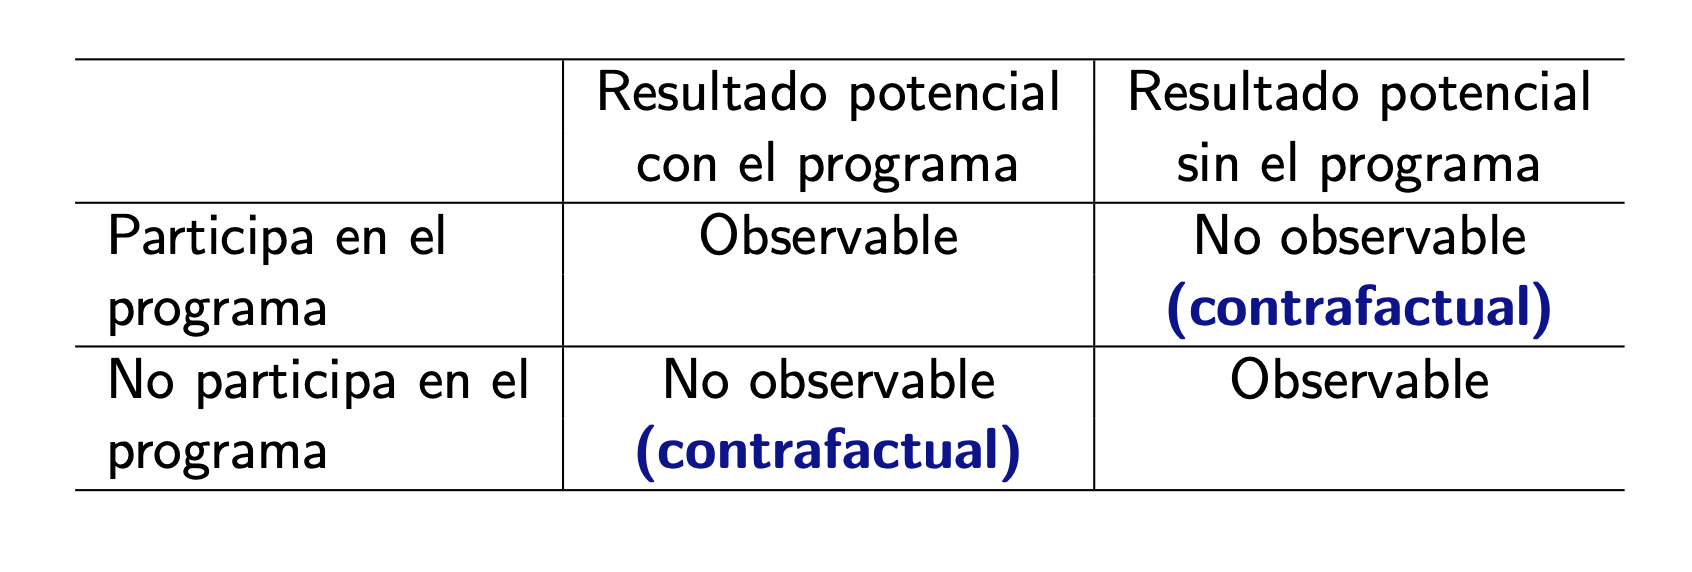
\includegraphics[width=0.9\textwidth,height=\textheight]{figs/resultados_potenciales}
\end{frame}

\begin{frame}{Una solución\ldots{}}
\protect\hypertarget{una-soluciuxf3n}{}
\pause
\center


\includegraphics[width=1\textwidth,height=\textheight]{figs/volver_al_futuro}
\end{frame}

\hypertarget{identificaciuxf3n}{%
\section{Identificación}\label{identificaciuxf3n}}

<<<<<<< Updated upstream
\begin{frame}{Efecto causal medio}
\protect\hypertarget{efecto-causal-medio}{}
\begin{itemize}
\tightlist
\item
  Aunque no podemos medir el efecto causal individual,
  \(\tau_i = Y_i(1)-Y_i(0)\), podemos asignar aleatoriamente sujetos a
  las condiciones de tratamiento y control para estimar el
  \textbf{efecto causal medio}, \(\bar{\tau}_i\):
\end{itemize}

\centering

\(\overline{\tau_i} = \frac{1}{N} \sum_{i=1}^N ( Y_i(1)-Y_i(0) ) = \overline{Y_i(1)-Y_i(0)}\)

\begin{itemize}
\tightlist
\item
  El efecto causal medio también se conoce como efecto medio del
  tratamiento (ATE).
\end{itemize}
\end{frame}

\begin{frame}{Estimandos y preguntas causales}
\protect\hypertarget{estimandos-y-preguntas-causales}{}
\begin{itemize}
\item
  Antes de hablar de la aleatorización y de cómo nos permite estimar la
  ATE, tener en cuenta que el ATE es un tipo de estimando.
\item
  Un estimando es una cantidad sobre la que se quiere aprender (a partir
  de los datos). Es el objetivo de su investigación que \emph{tu}
  eliges.
\item
  Ser preciso sobre la pregunta de investigación significa ser preciso
  sobre el estimando. Para las preguntas causales, esto significa
  especificar:

  \begin{itemize}
  \tightlist
  \item
    El resultado
  \item
    Las condiciones de tratamiento y control
  \item
    La población de estudio
  \end{itemize}
\end{itemize}
\end{frame}

\begin{frame}{Otros tipos de estimandos}
\protect\hypertarget{otros-tipos-de-estimandos}{}
\begin{itemize}
\item
  El ATE para un subgrupo concreto, también conocido como efecto medio
  condicional del tratamiento (CATE)
\item
  Las diferencias en los CATE: diferencias en el efecto medio del
  tratamiento para un grupo en comparación con otro grupo.
\item
  El ATE sólo para las unidades tratadas, también conocido como ATT
  (efecto medio del tratamiento sobre los tratados).
\item
  El ATE local (LATE). ``Local'' = aquéllas cuyo estado de tratamiento
  cambiaría por un estímulo en un diseño de aliento (alias CACE,
  ``\emph{complier average causal effect}'') o aquéllas en la vecindad
  de una discontinuidad para un diseño de regresión discontinua.
\end{itemize}
\end{frame}

\begin{frame}{Estrategia de identificación}
\protect\hypertarget{estrategia-de-identificaciuxf3n}{}
=======
\begin{frame}{Problema fundamental de la inferencia causal}
\protect\hypertarget{problema-fundamental-de-la-inferencia-causal-2}{}
>>>>>>> Stashed changes
Una estrategia de identificación implica sortear el \emph{problema
fundamental de la inferencia causal}. Lo que \textcolor{red}{NO} podemos
estimar:

\[
\begin{aligned}
E[Y_{i}(1) | T = 1] & - E[Y_{i}(0) | T = 0]
\end{aligned}
\] \pause

\center

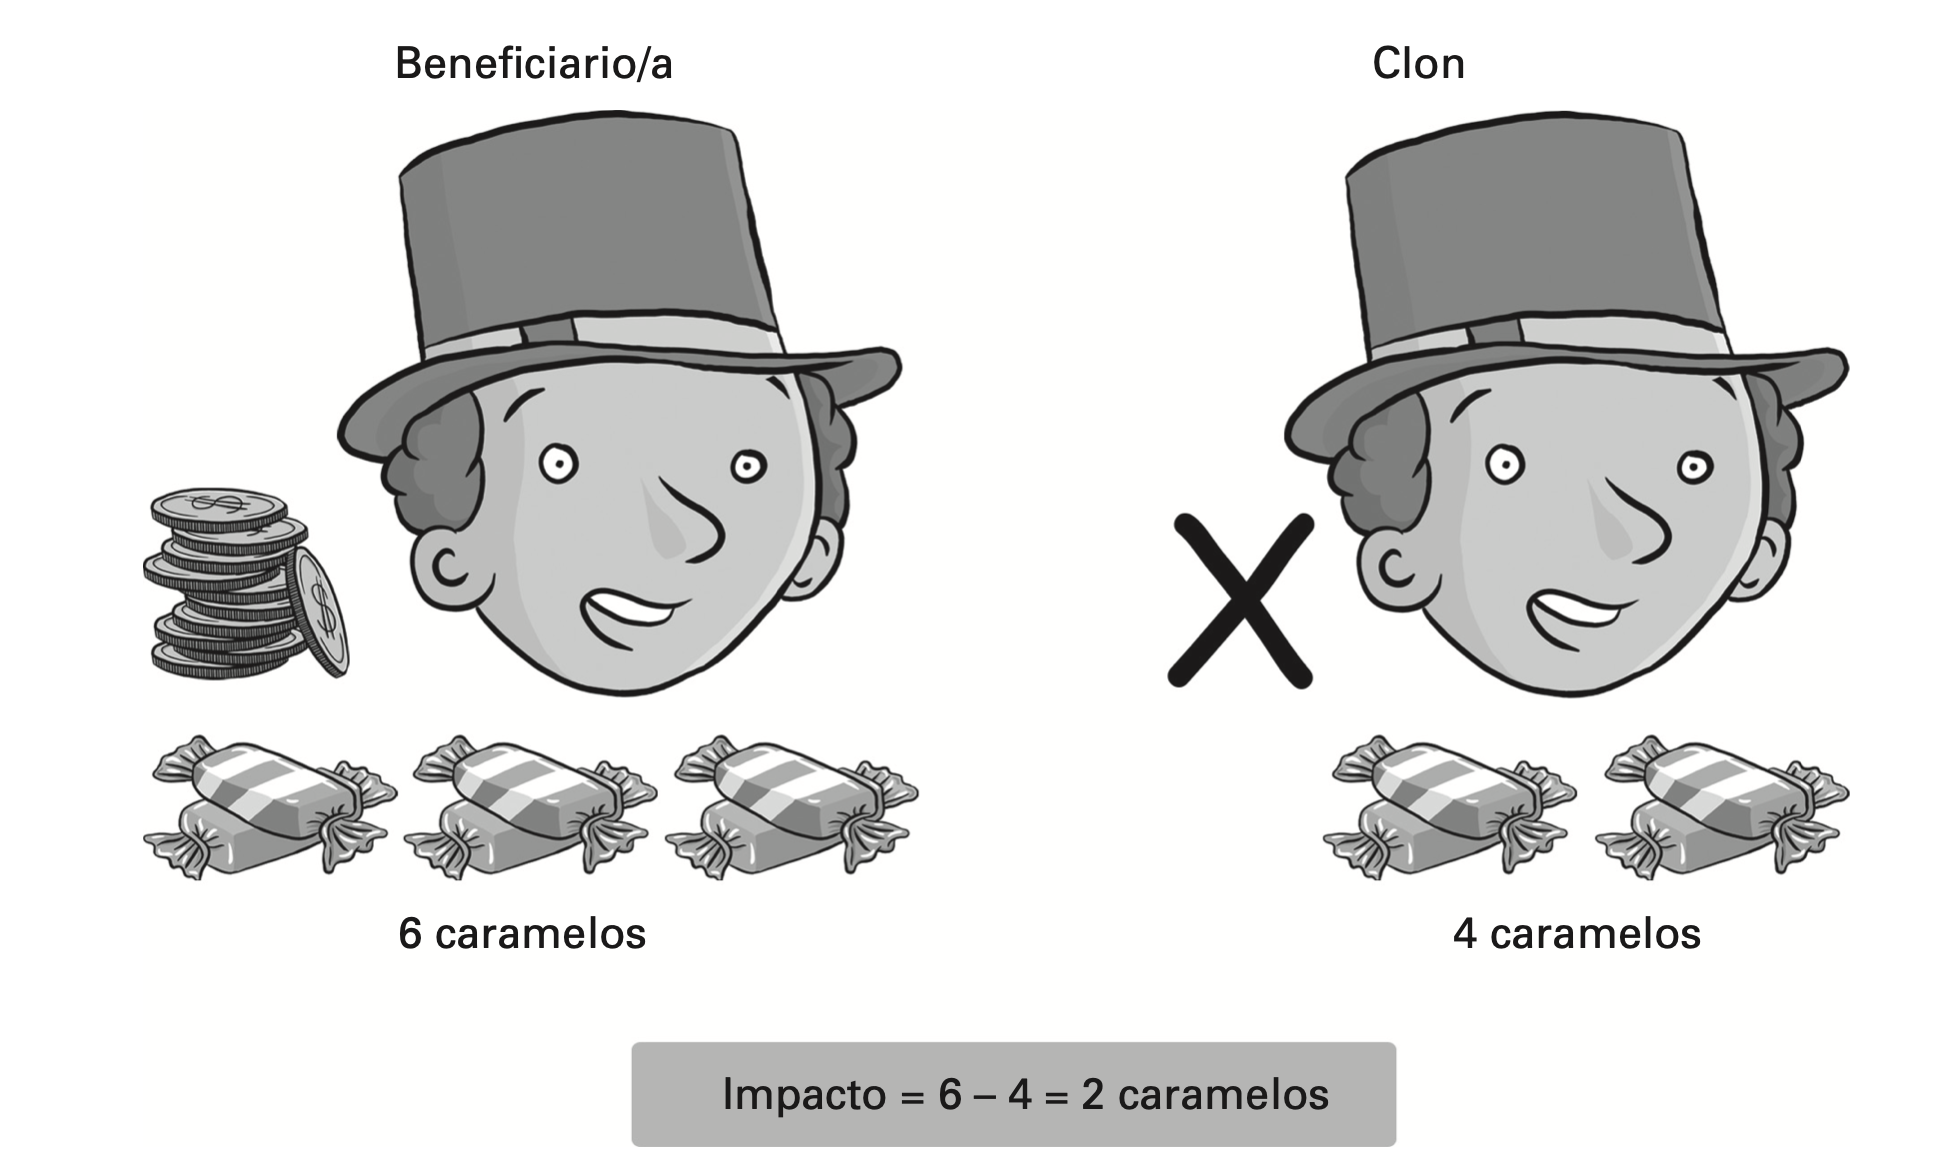
\includegraphics[width=0.49\textwidth,height=\textheight]{figs/clon_contrafactual}
\end{frame}

\begin{frame}{Estrategia de identificación}
<<<<<<< Updated upstream
\protect\hypertarget{estrategia-de-identificaciuxf3n-1}{}
=======
\protect\hypertarget{estrategia-de-identificaciuxf3n}{}
>>>>>>> Stashed changes
\begin{itemize}
\tightlist
\item
  La idea central es estimar el contrafactual \(Y_{i}(0)\) \pause
\item
  Esto no puede hacerce para cada unidad que fue trtatada \pause
\item
  Se puede usar un grupo de comparación y estimar una media
  \(E[Y_{i} | T = 0]\)
\end{itemize}
\end{frame}

\begin{frame}{Estrategia de identificación}
<<<<<<< Updated upstream
\protect\hypertarget{estrategia-de-identificaciuxf3n-2}{}
=======
\protect\hypertarget{estrategia-de-identificaciuxf3n-1}{}
>>>>>>> Stashed changes
Un grupo de comparación válido:

\begin{enumerate}
[(1)]
\tightlist
\item
  Tiene las mismas características, en promedio, que el grupo de
  tratamiento en ausencia del tratamiento; \pause
\item
  no es afectado por el tratamiento; \pause
\item
  reaccionaría al tratamiento de la misma manera que el grupo de
  tratamiento, si fuera objeto del tratamiento \pause
\end{enumerate}

\center

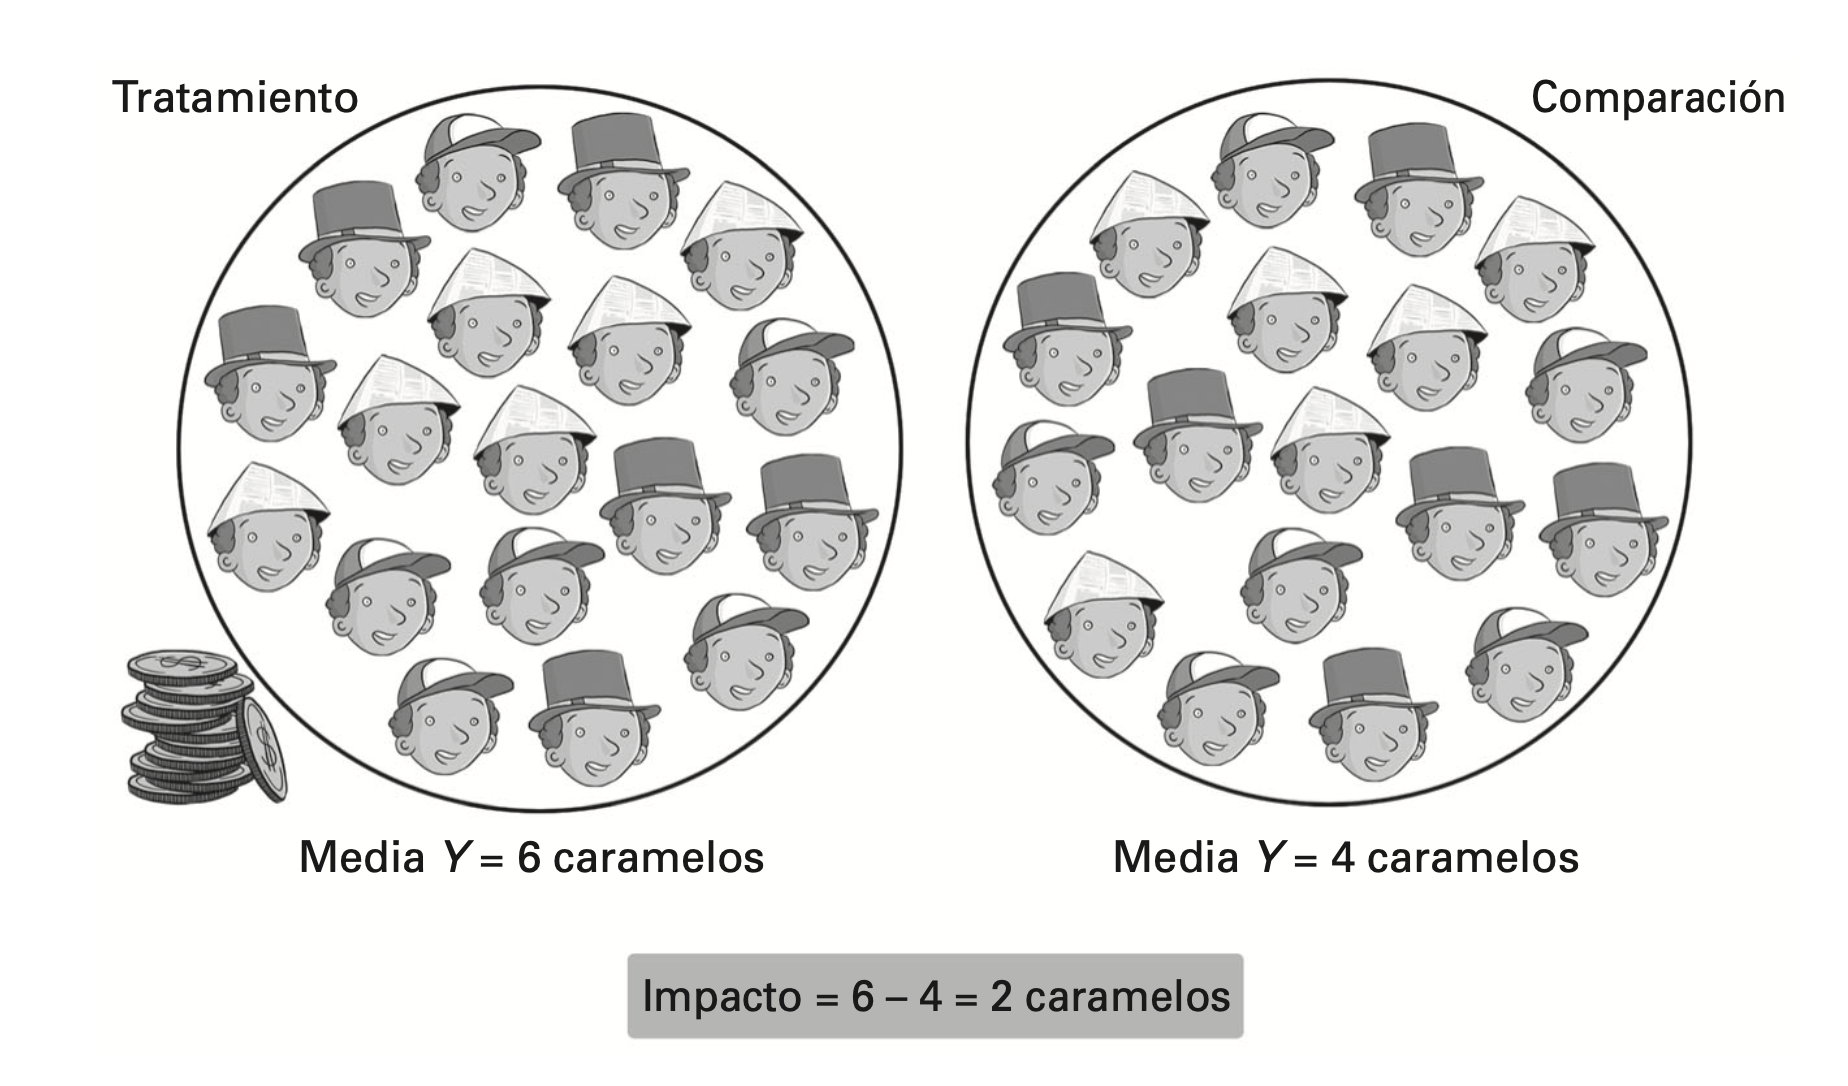
\includegraphics[width=0.6\textwidth,height=\textheight]{figs/comparacion}
\end{frame}

\begin{frame}{Supuesto de independencia}
\protect\hypertarget{supuesto-de-independencia}{}
La identificación descansa en el supuesto de independencia entre el
\textbf{status de tratamiento} y los \textbf{resultados potenciales}

\[ Y_{i}(1), Y_{i}(0) \perp T_i \]

\pause

En ese caso, entonces:

\[
\begin{aligned}
ATE &=  E[Y_{i1} - Y_{i0}] \\
    &=  E[Y_{i1}] - E[Y_{i0}] \\
    &=  E[Y_{i} | T=1 ] - E[Y_{i} | T=0]
\end{aligned}
\]

La expectativa de resultados potenciales no-observados es igual la
expectativa condicional en la asignación del tratamiento.
\end{frame}

\begin{frame}{}
\protect\hypertarget{section}{}
¿Cuándo podemos justificar que el supuesto de independencia entre
tratamiento y resultados potenciales se sostiene?

\begin{itemize}
\tightlist
\item
  Distintas \textbf{\emph{estrategias de identificación}}
\end{itemize}

\vspace{16pt}

\begin{quote}
``To ask what is your identification strategy is to ask what research
design (and assumptions) one intends to use for the identification of a
causal effect.'' (Keele, 2015)
\end{quote}
\end{frame}

\hypertarget{experimentos}{%
\section{Experimentos}\label{experimentos}}

\begin{frame}{Experimentos aleatorizados}
\protect\hypertarget{experimentos-aleatorizados}{}
Estándar de oro de las estrategias de identificación

Los sujetos son asignados a \(D_{i}\) en forma \textbf{aleatoria}

El investigador impone la independencia entre la \textbf{condición de
tratamiento} y los \textbf{resultados potenciales} \pause

Tratados y no tratados son en expectativa iguales en:

\begin{itemize}
\tightlist
\item
  características observables
\item
  características no observables
\end{itemize}
\end{frame}

\begin{frame}{Diseños}
\protect\hypertarget{diseuxf1os}{}
Variedad de tipos de experimentos, por ej.:

\begin{itemize}
\tightlist
\item
  Experimentos de campo

  \begin{itemize}
  \tightlist
  \item
    Aleatorización de intervenciones (programas)
  \item
    ``Nudges'' (o información) \pause
  \end{itemize}
\item
  Experimentos de laboratorio \pause
\item
  Experimentos de encuesta
\item
  Experimentos naturales
\end{itemize}

\pause

Número de condiciones de tratamiento:

\begin{itemize}
\tightlist
\item
  Tratamiento y Control
\item
  Múltiples ``brazos'' (\(T_1\), \(T_2\), \(C\)) \pause
\item
  Factoriales (2 x 2) \pause
\item
  Otras estrategias de aleatorización
\end{itemize}

\pause

Forma de asignación al tratamiento:

\begin{itemize}
\tightlist
\item
  Fuerza bruta\pause
\item
  Aliento (promoción)
\end{itemize}
\end{frame}

\begin{frame}{Nudges con tres brazos}
\protect\hypertarget{nudges-con-tres-brazos}{}
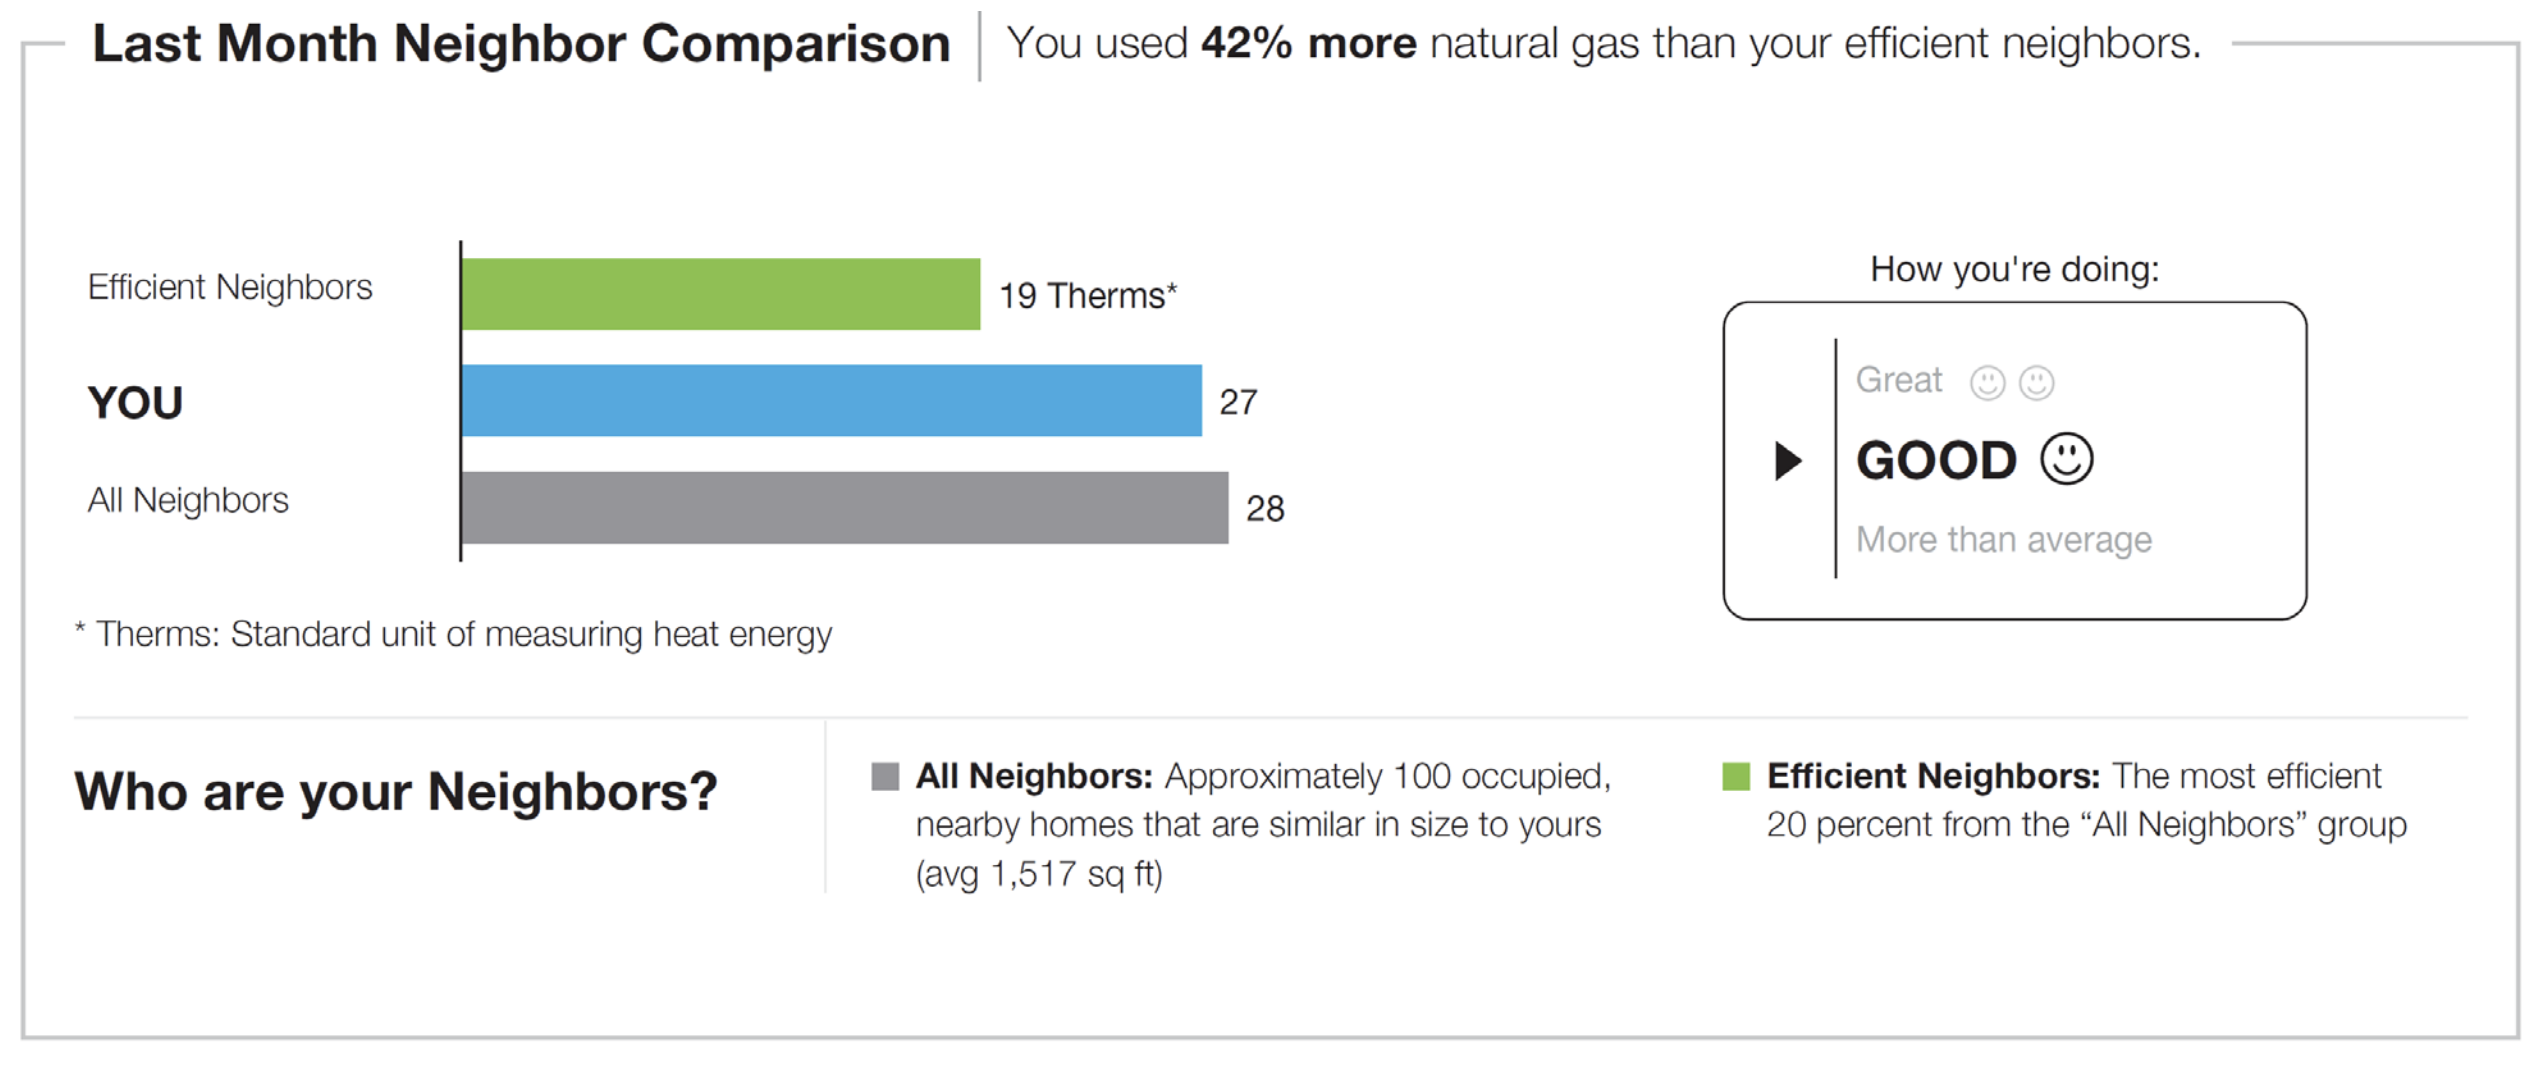
\includegraphics[width=0.9\textwidth,height=\textheight]{figs/electricity_nudge}

\begin{scriptsize}
Schultz et al. (2007) 
\end{scriptsize}
\end{frame}

\begin{frame}{Experimento de campo con diseño factorial}
\protect\hypertarget{experimento-de-campo-con-diseuxf1o-factorial}{}
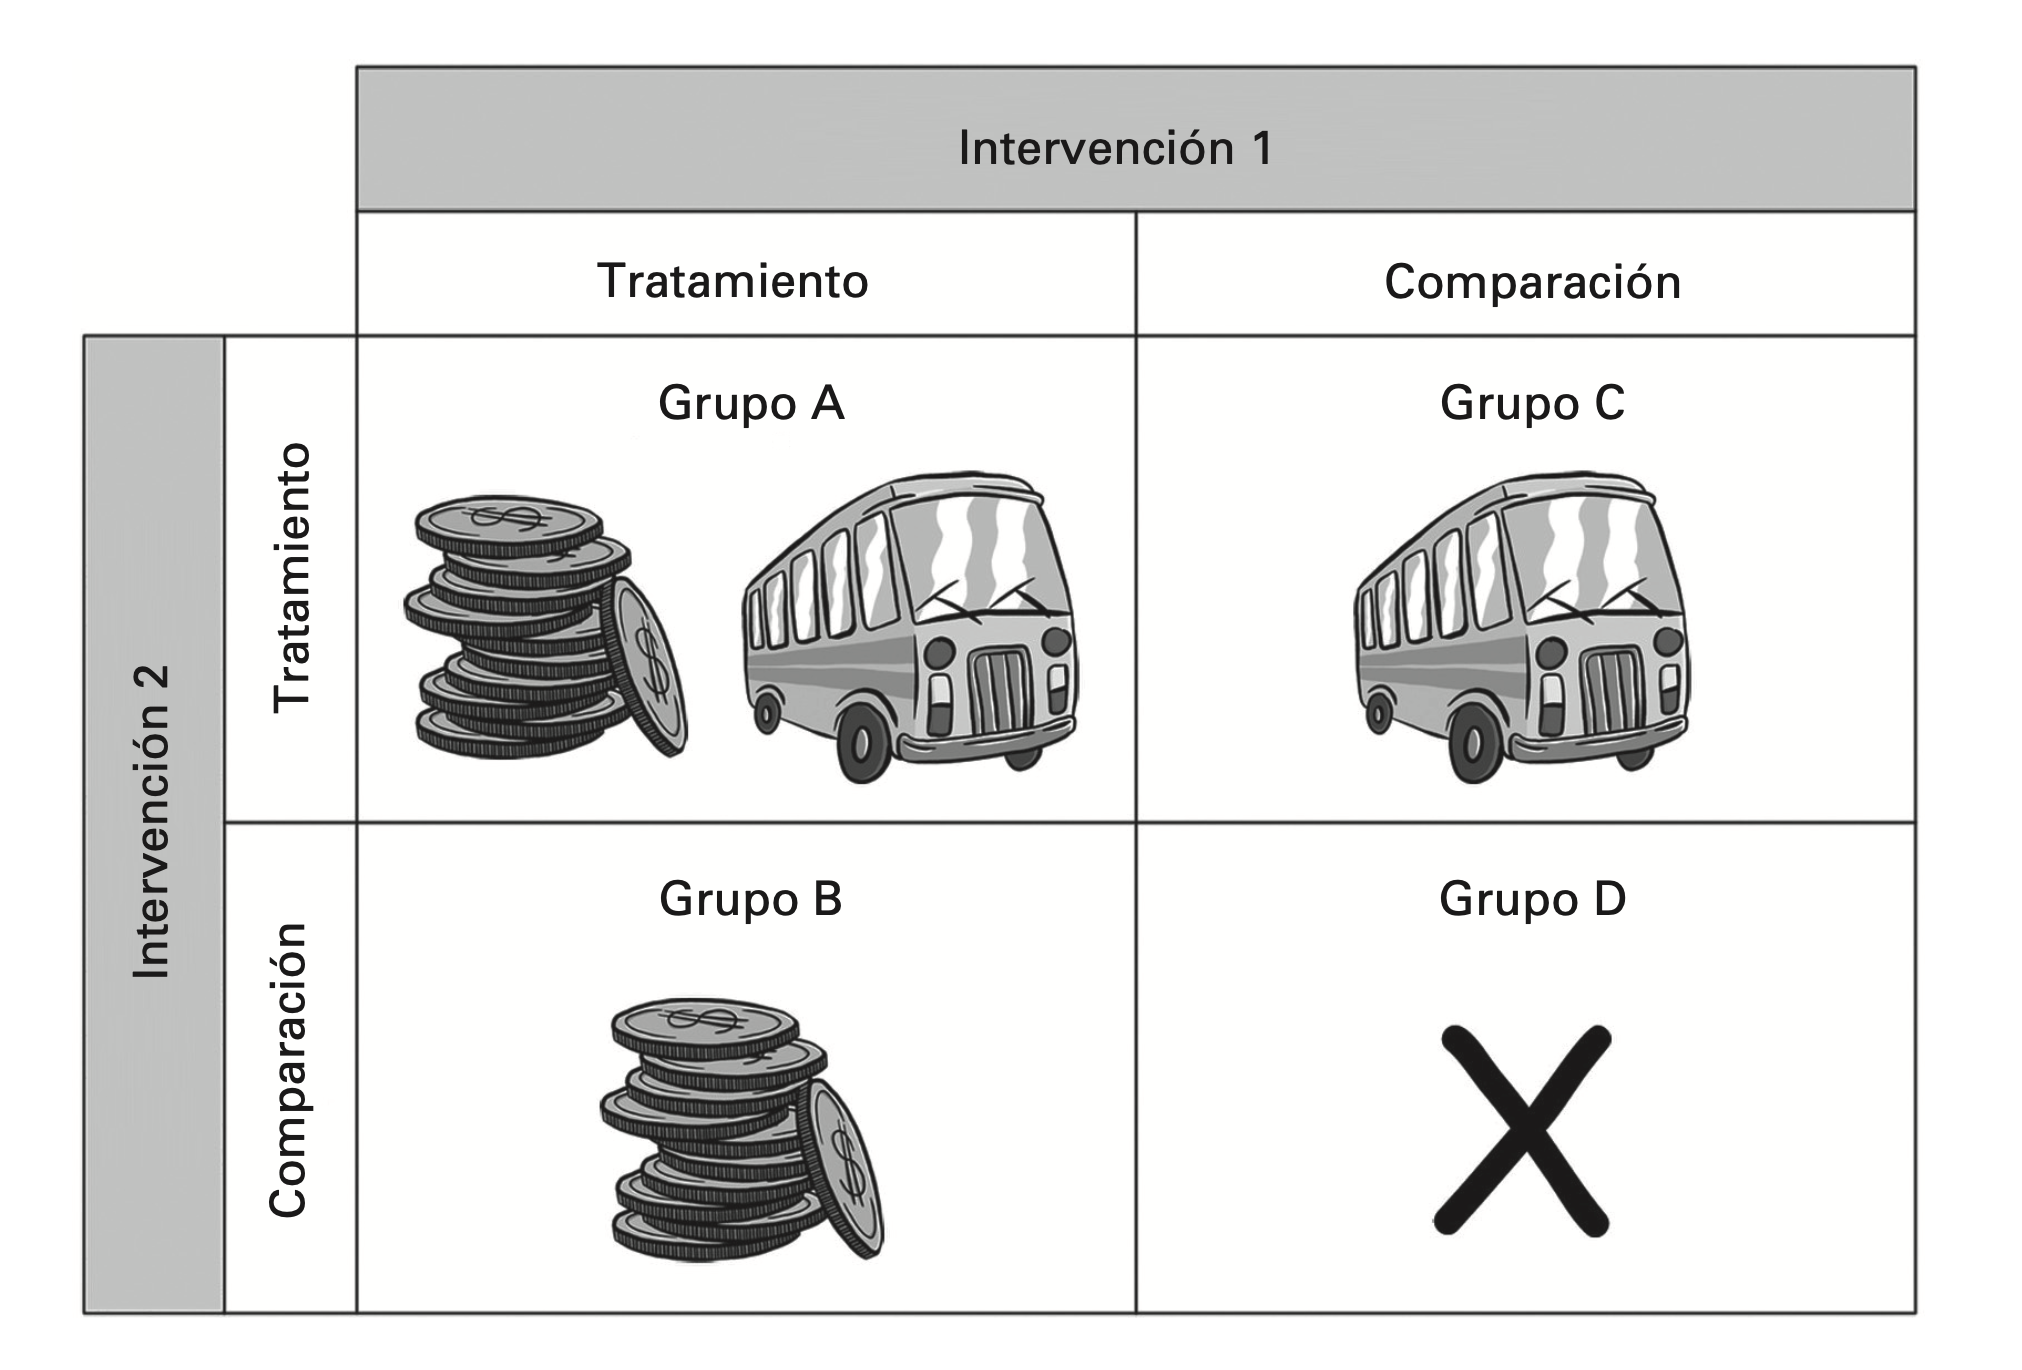
\includegraphics[width=0.9\textwidth,height=\textheight]{figs/dos_int2}
\end{frame}

\begin{frame}{Fortalezas y limitaciones}
\protect\hypertarget{fortalezas-y-limitaciones}{}
Fortaleza:

\begin{itemize}
\tightlist
\item
  Validez interna
\end{itemize}

Limitaciones:

\begin{itemize}
\tightlist
\item
  Desgaste
\item
  Efecto derrame
\item
  Ética
\item
  Validez externa
\end{itemize}
\end{frame}

\begin{frame}{Validez interna y externa}
\protect\hypertarget{validez-interna-y-externa}{}
\begin{columns}
\begin{column}{0.4\textwidth}

\begin{scriptsize}
\textbf{Validez externa}: la \textit{muestra} de la evaluación representa con precisión a la población de unidades elegibles.

\vspace{16pt}


\textbf{Validez interna}: El impacto estimado del programa es el impacto libre de todos los demás factores de confusión potenciales (o, en otras palabras, que el grupo de comparación represente una estimación precisa del contrafactual de modo que se estime el verdadero impacto del programa).

\end{scriptsize}

\end{column}
\begin{column}{0.6\textwidth}


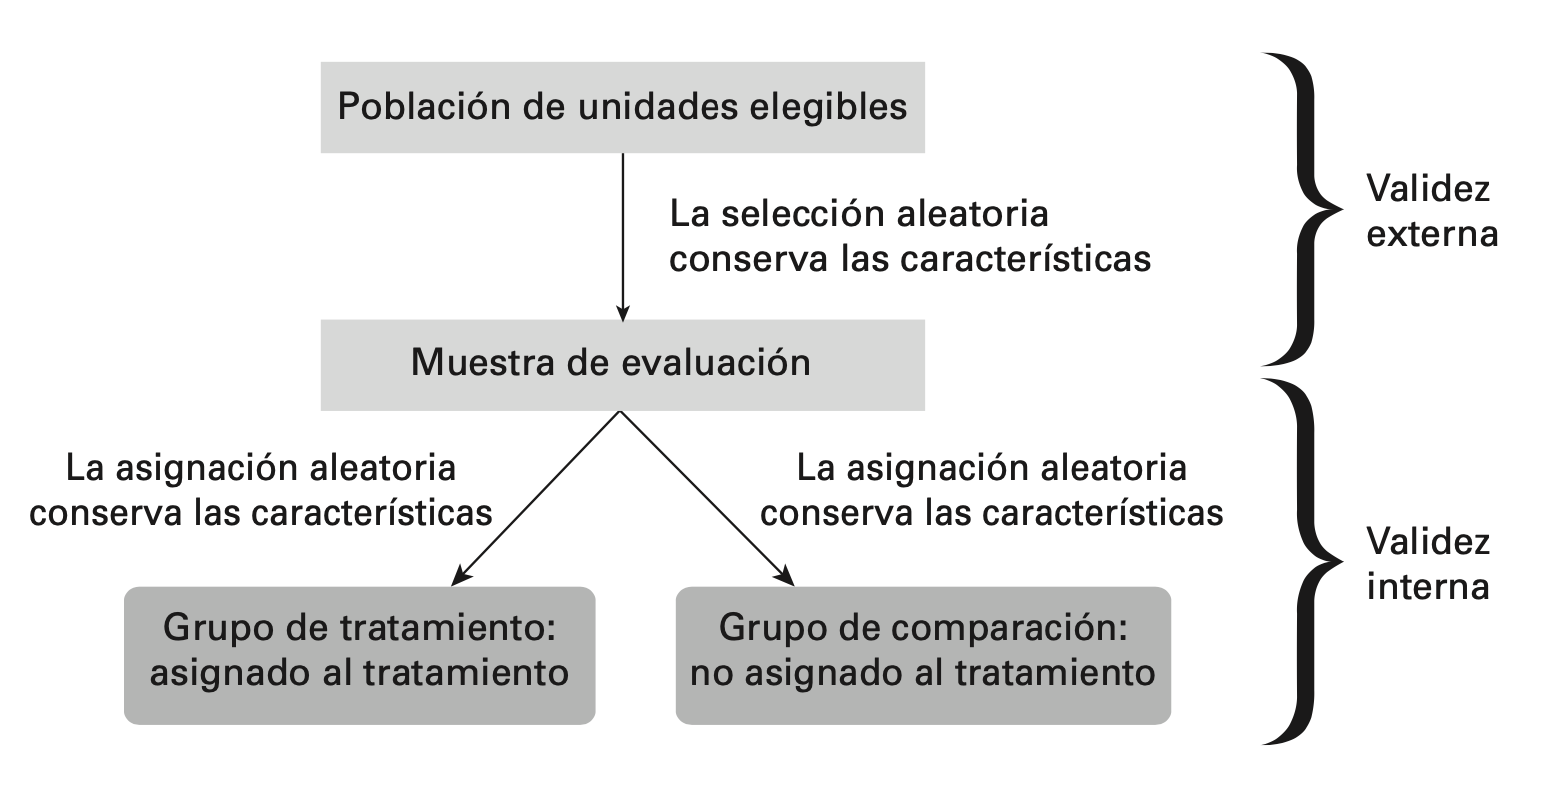
\includegraphics[width=1\textwidth]{figs/vive.png}

\begin{tiny}
Fuente: Gertler, et al. (2017).
\end{tiny}

\end{column}
\end{columns}
\end{frame}

\begin{frame}{Validez interna y externa}
\protect\hypertarget{validez-interna-y-externa-1}{}
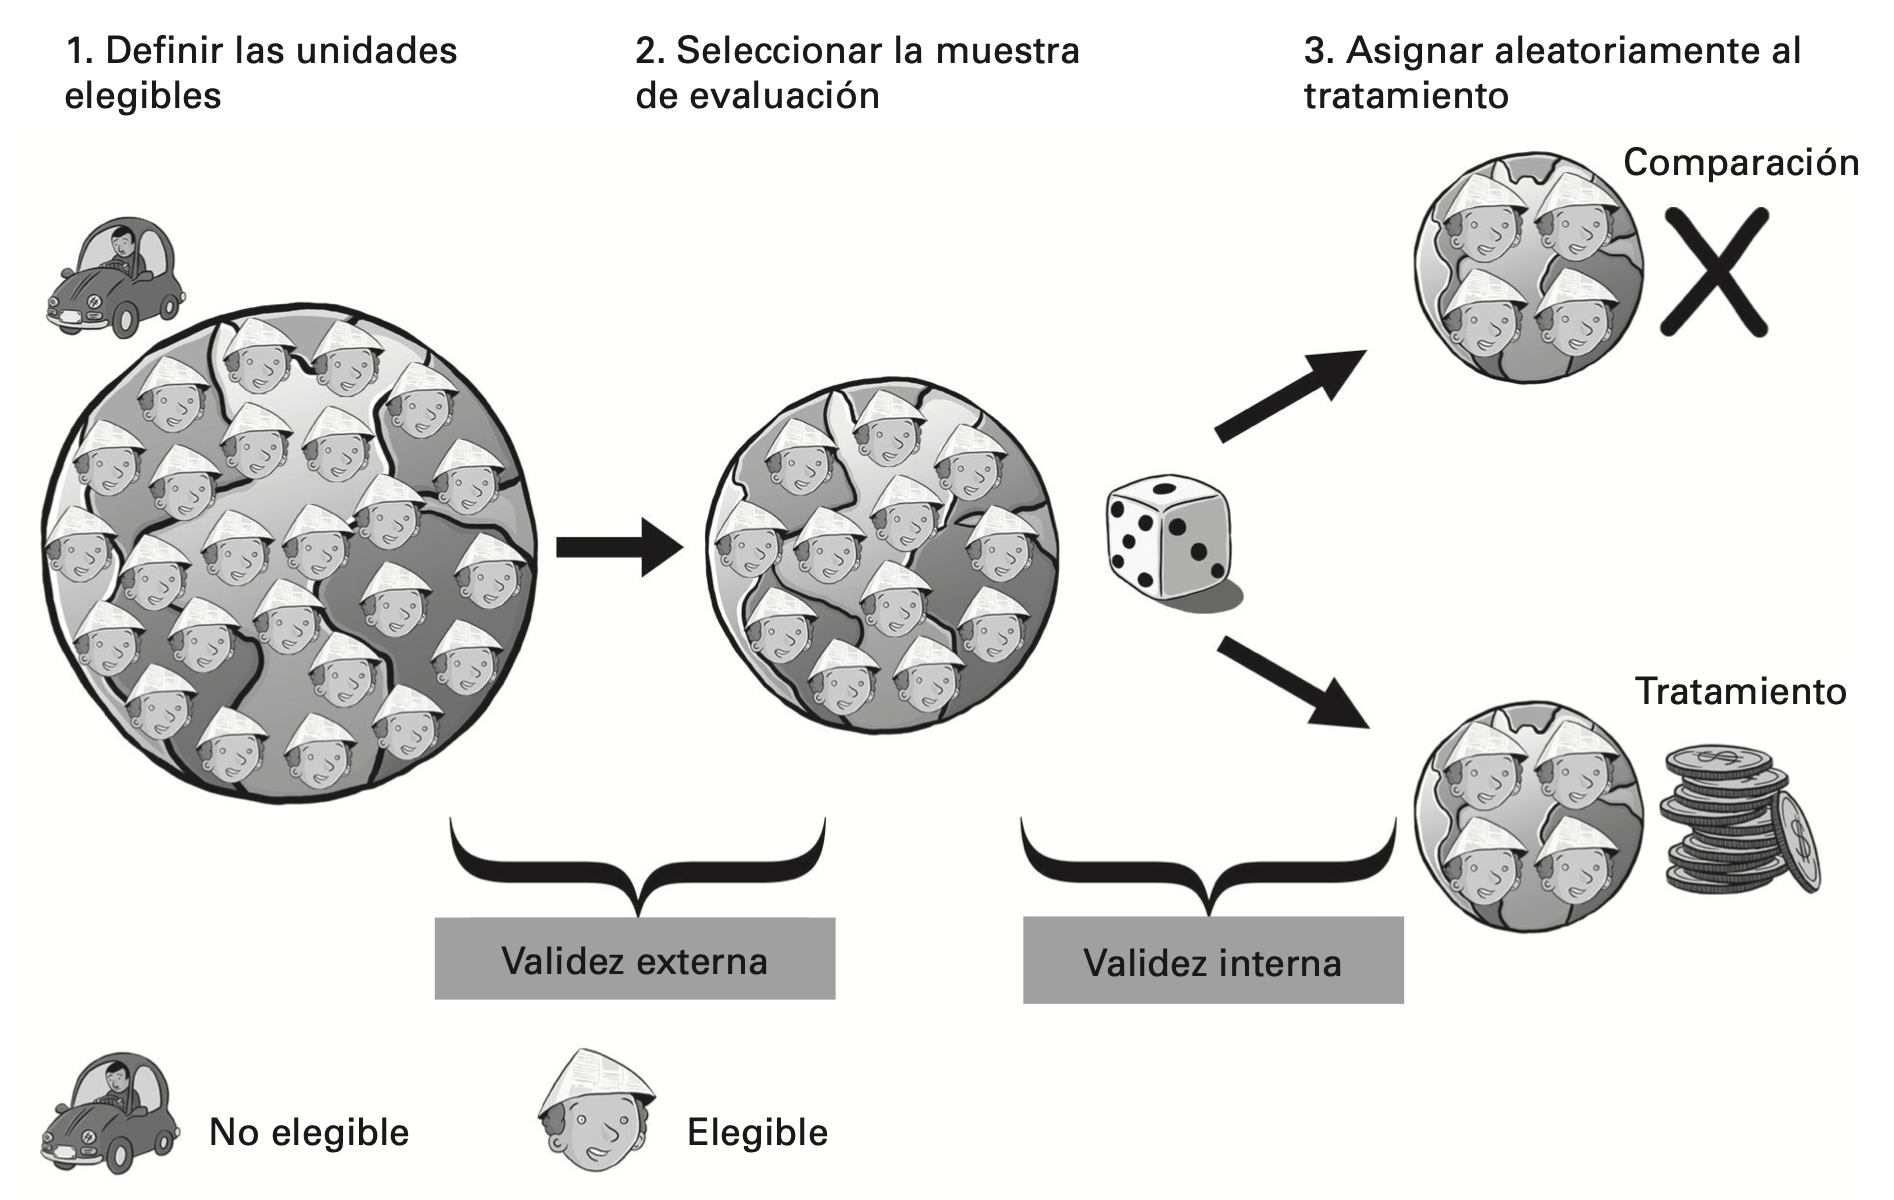
\includegraphics{figs/vive2.png}

\begin{tiny}
Fuente: Gertler, et al. (2017).
\end{tiny}
\end{frame}

\begin{frame}{Respuestas a la ``crisis'' de validez externa}
\protect\hypertarget{respuestas-a-la-crisis-de-validez-externa}{}
\begin{itemize}
\tightlist
\item
  Investigar la existencia de efectos de tratamiento heterogéneos

  \begin{itemize}
  \tightlist
  \item
    Interaccion entre \(T_i\) y características de los sujetos \(X_i\)
    (sexo, edad, educación, lugar de residencia, etc.)
  \item
    Depende de observables en \(X\). \pause \vspace{16pt}
  \end{itemize}
\item
  Replicación
\end{itemize}
\end{frame}

\begin{frame}{Replicación}
\protect\hypertarget{replicaciuxf3n}{}

\includegraphics[width=0.9\textwidth,height=\textheight]{figs/metaketa.png}
\href{https://egap.org/metaketa}{Ver proyectos Metaketa de EGAP aquí}
\end{frame}

\begin{frame}{Replicación}
\protect\hypertarget{replicaciuxf3n-1}{}
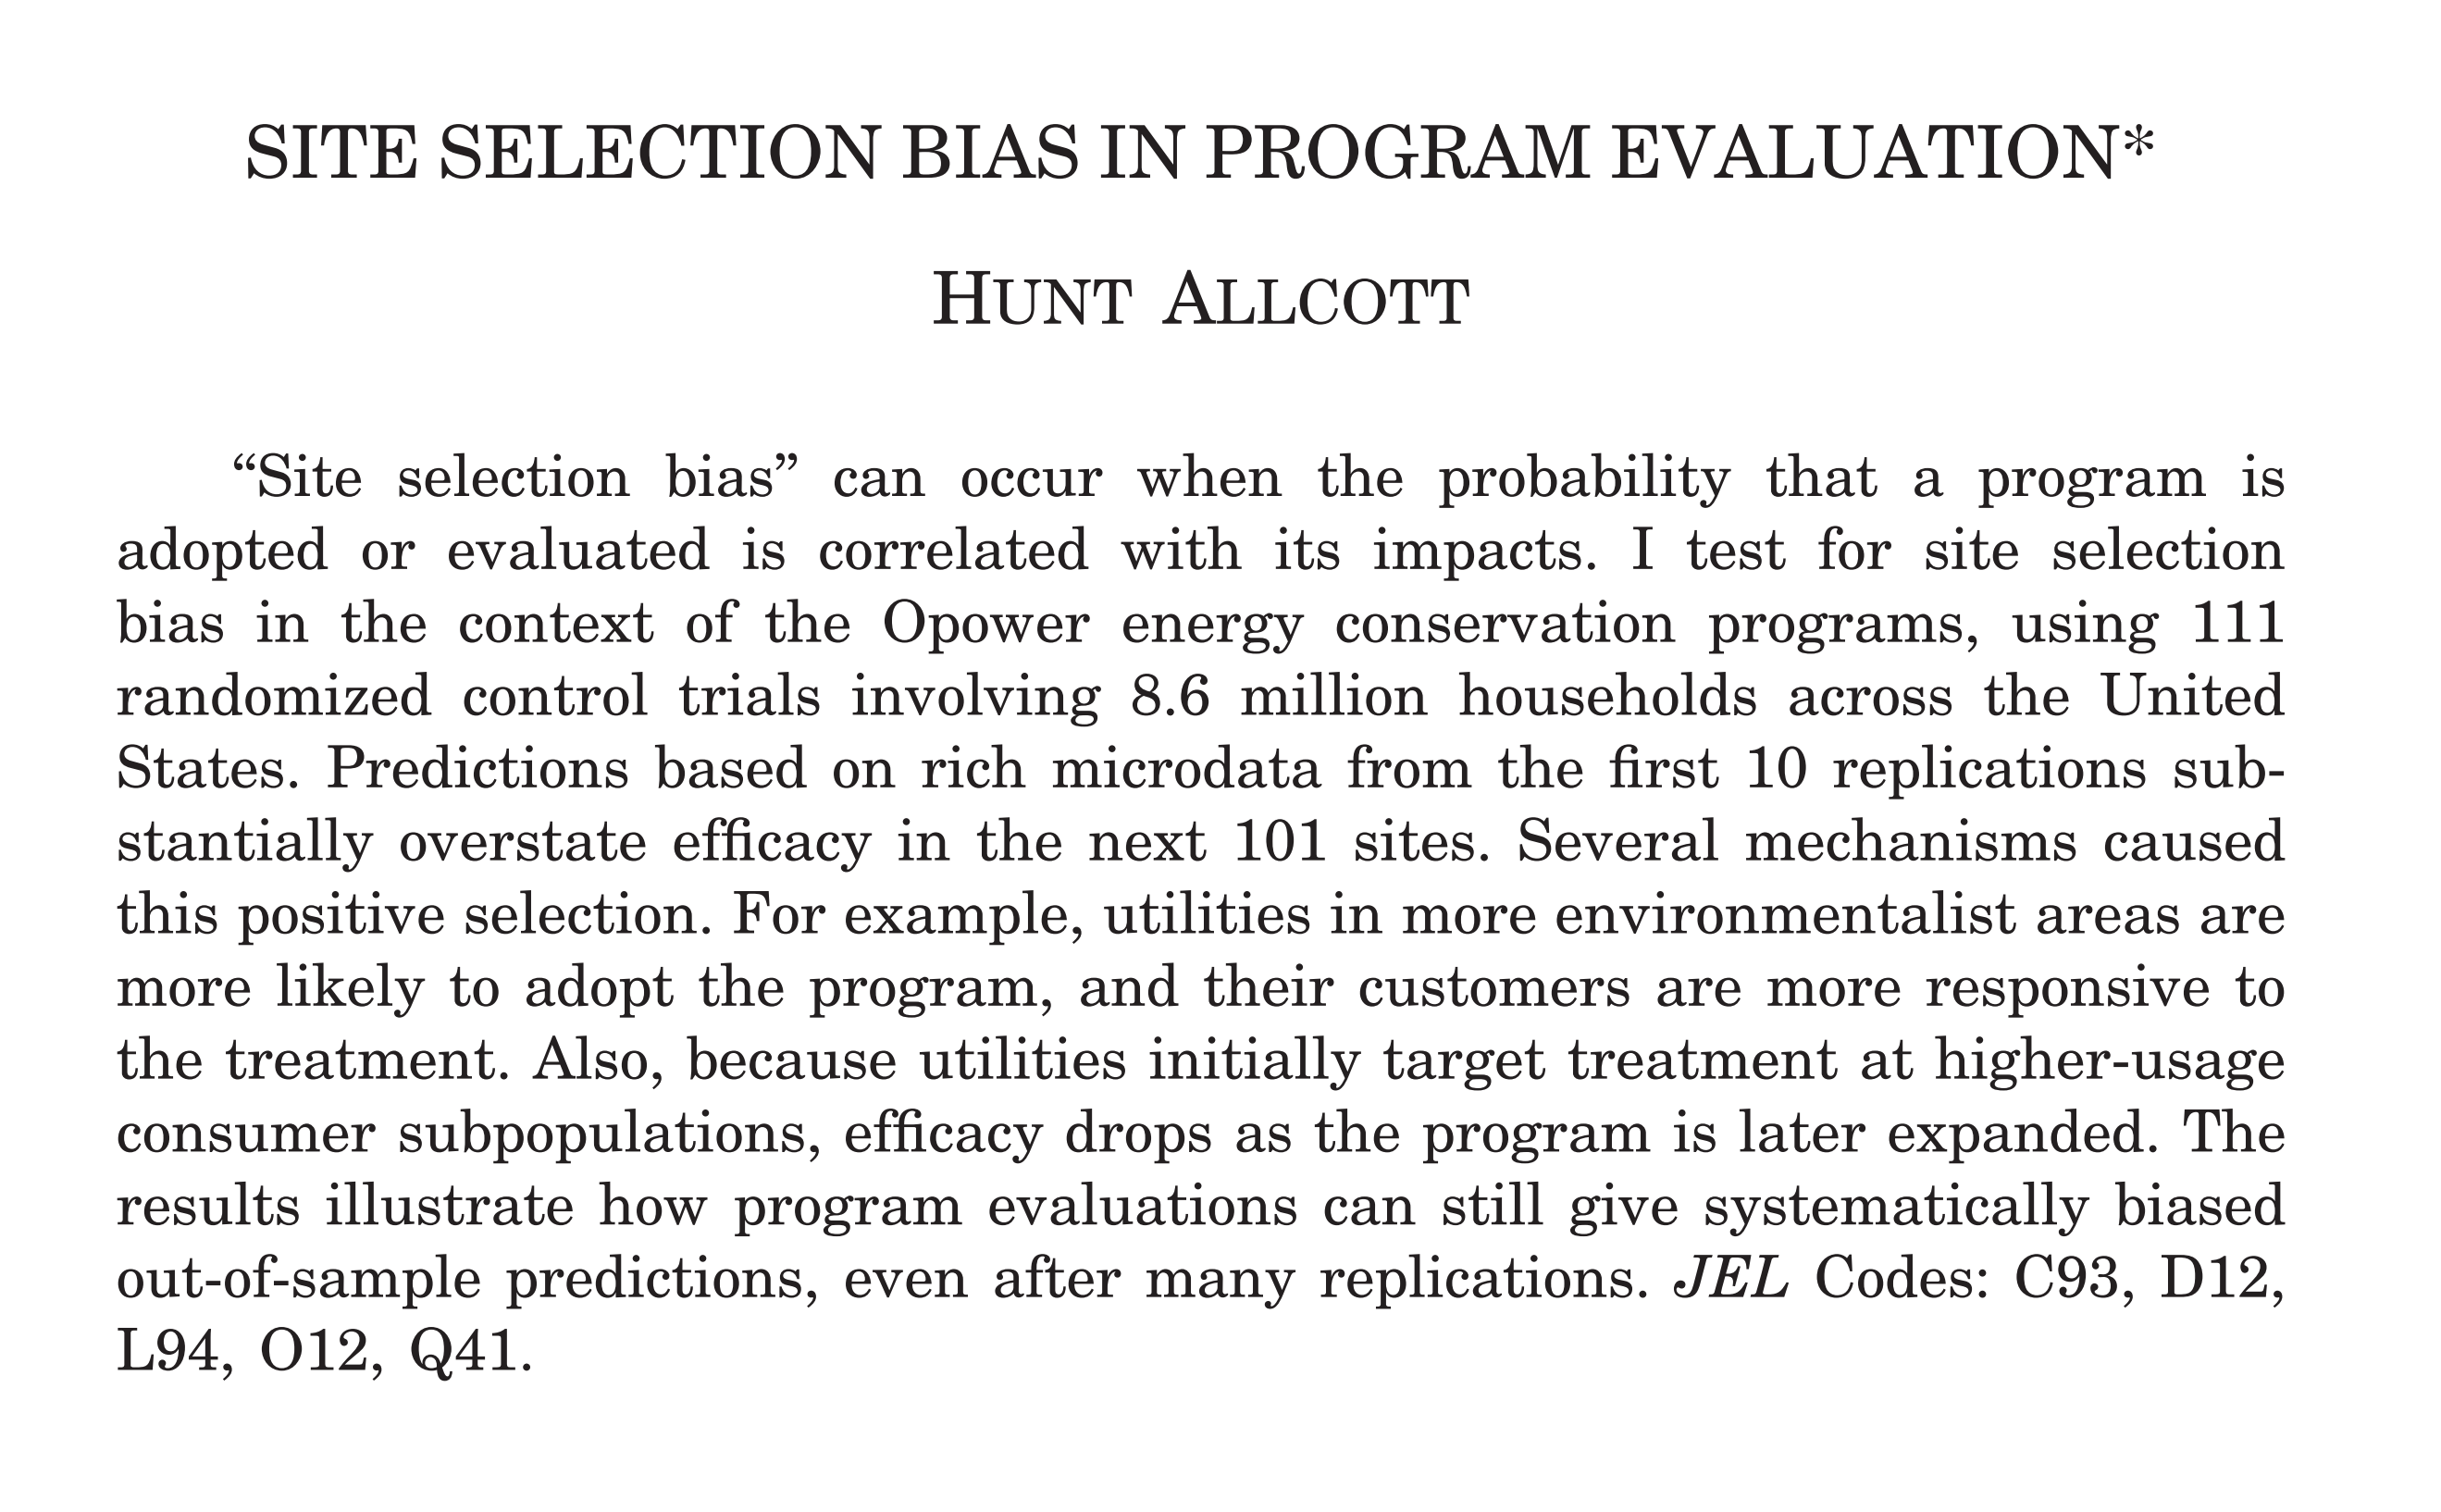
\includegraphics[width=0.9\textwidth,height=\textheight]{figs/allcott_selectionbias.png}

\begin{tiny}
Allcott, H. (2015). Site Selection Bias in Program Evaluation. The Quarterly Journal of Economics, 130(3), 1117–1165. https://doi.org/10.1093/qje/qjv015
\end{tiny}
\end{frame}

\begin{frame}{Replicación y sesgos de selección}
\protect\hypertarget{replicaciuxf3n-y-sesgos-de-selecciuxf3n}{}
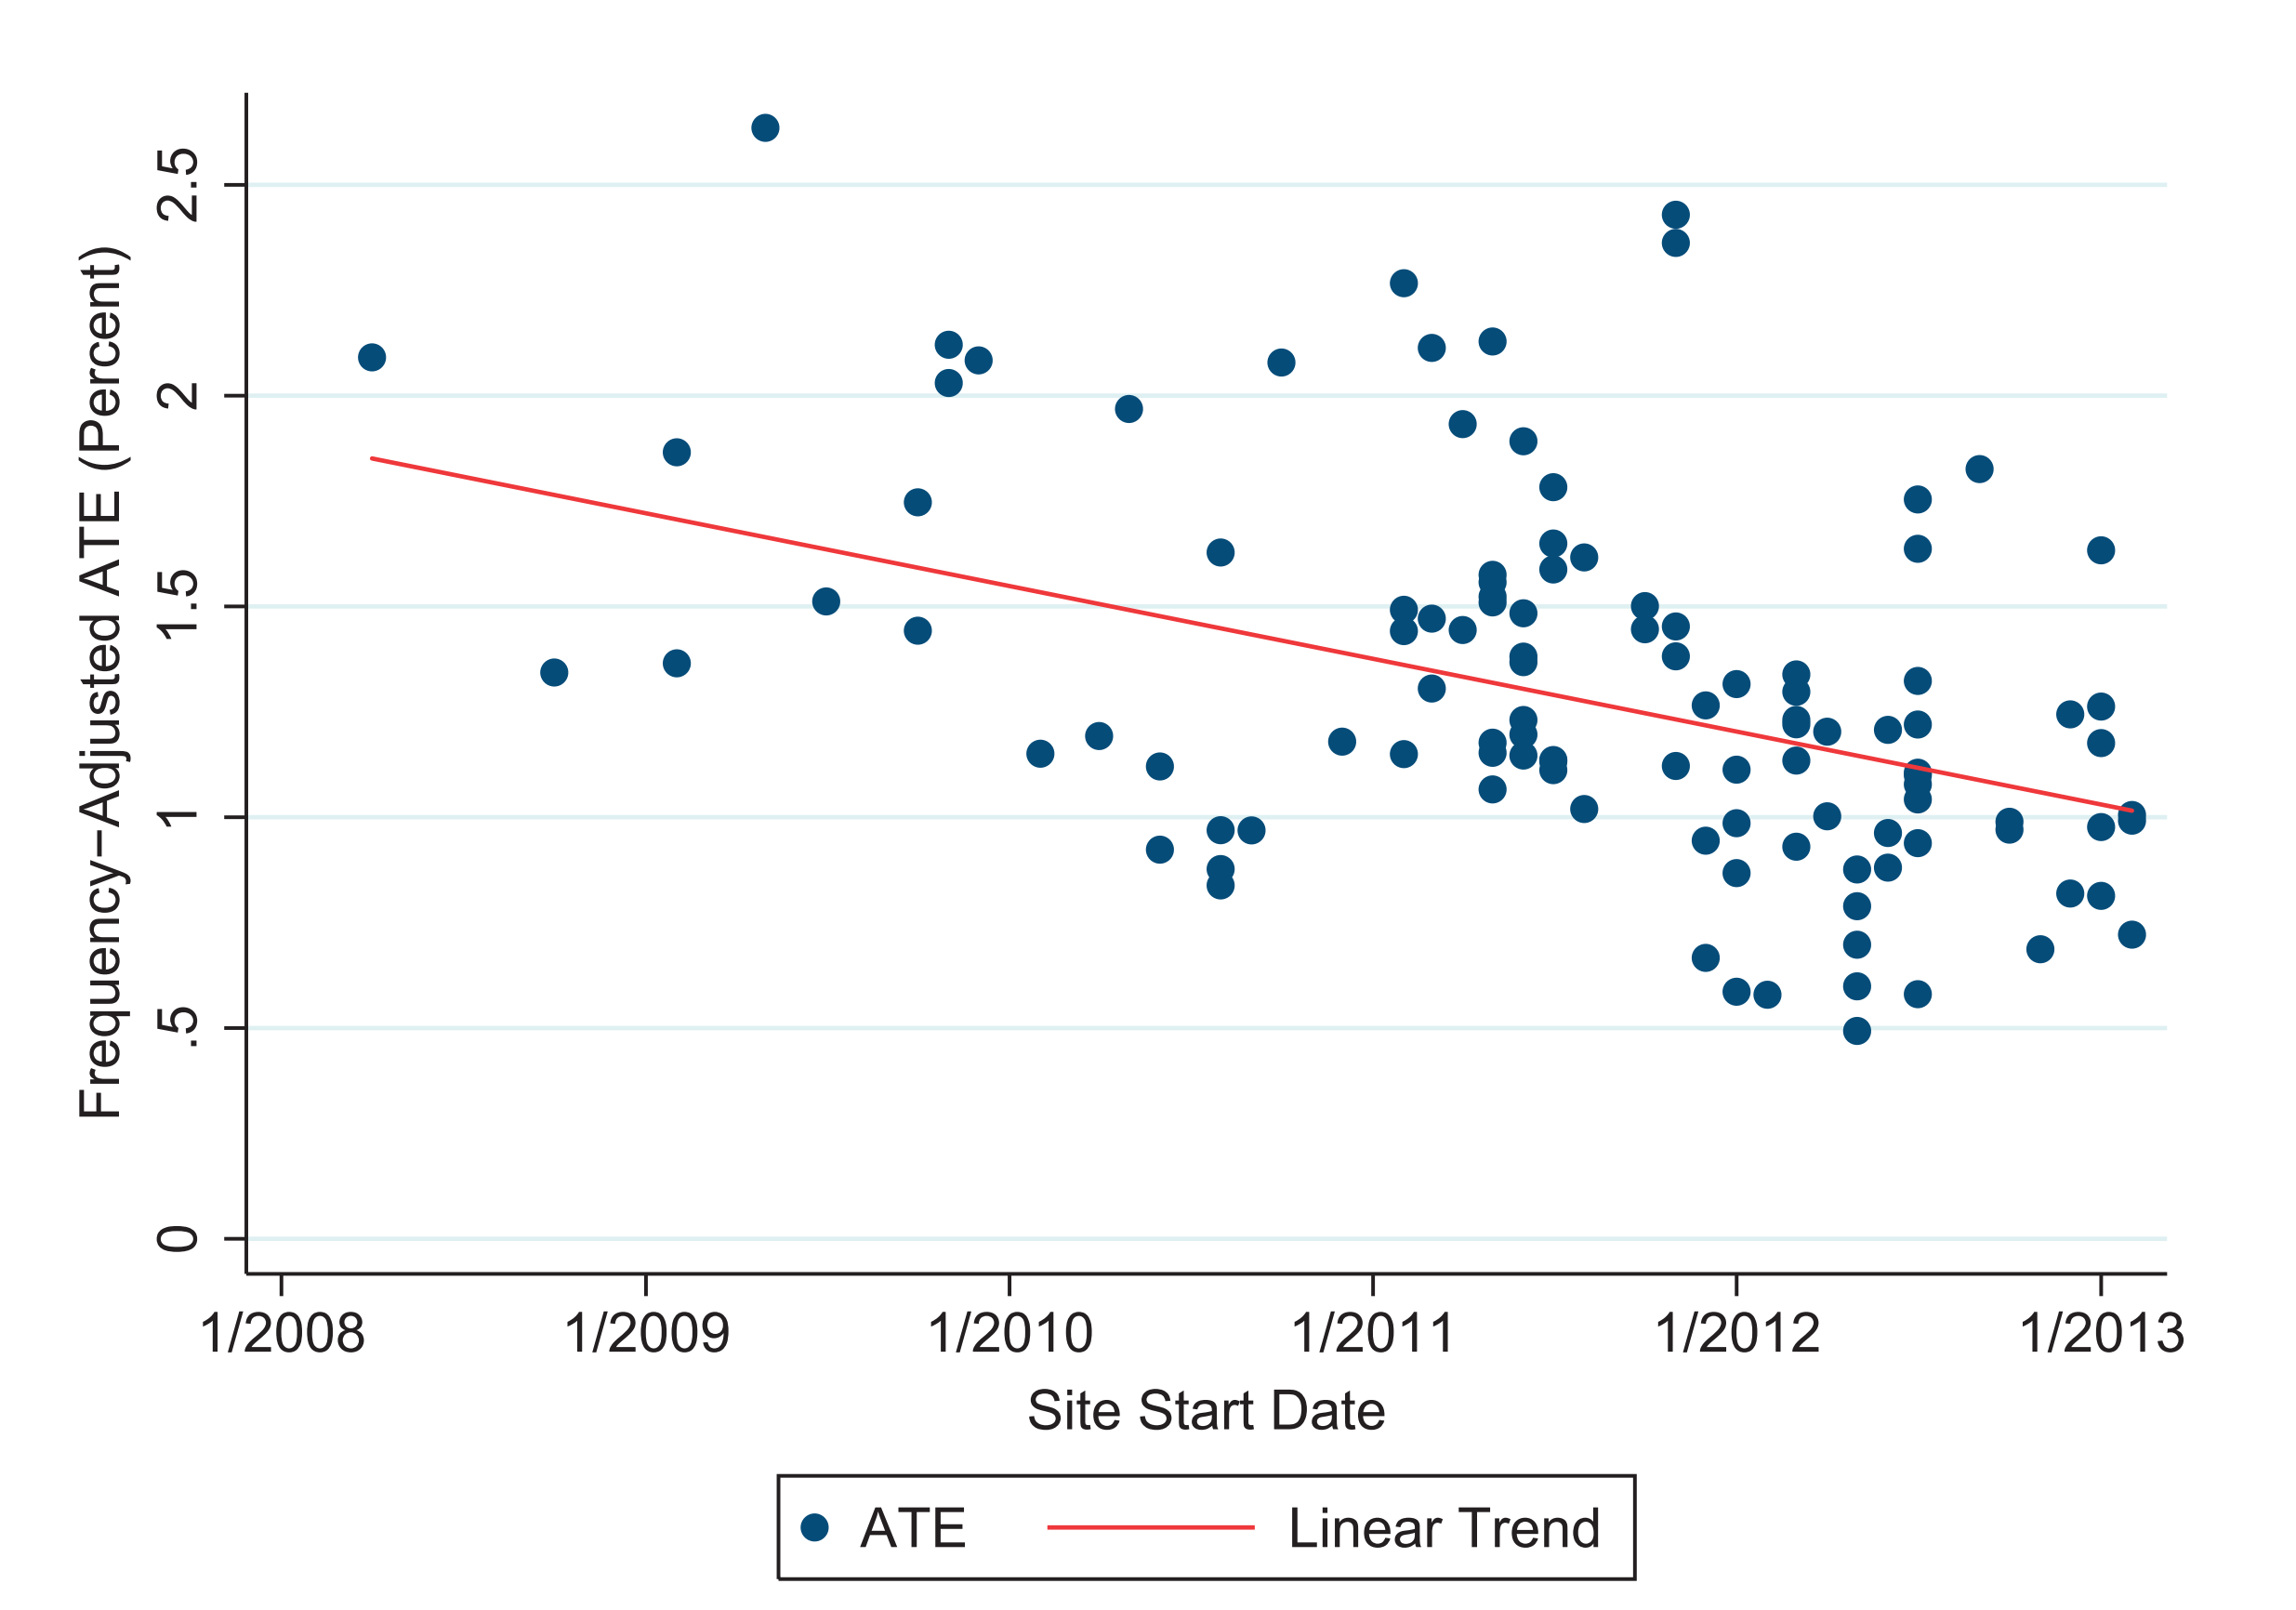
\includegraphics[width=0.9\textwidth,height=\textheight]{figs/allcott_selectionbias_plot.png}

\begin{tiny}
Allcott, H. (2015). Site Selection Bias in Program Evaluation. \textit{The Quarterly Journal of Economics}, 130(3), 1117–1165. https://doi.org/10.1093/qje/qjv015
\end{tiny}
\end{frame}

\begin{frame}{Experimentos Naturales}
\protect\hypertarget{experimentos-naturales}{}
\begin{itemize}
\item
  Una situación real que produce una asignación casual a un tratamiento
\item
  Esta situación genera una asignación al tratamiento \textbf{\emph{como
  si fuera aleatoria}} (as-if random)
\item
  Requiere una fuerte justificación
\end{itemize}
\end{frame}

\begin{frame}{}
\protect\hypertarget{section-1}{}

\includegraphics[width=0.9\textwidth,height=\textheight]{figs/angrist_NatExp.png}

\begin{tiny}
Angrist, Joshua, Eric Bettinger, Erik Bloom, Elizabeth King, and Michael Kremer. 2002. “Vouchers for Private Schooling in Colombia: Evidence from a Randomized Natural Experiment.” \textit{American Economic Review} 92 (5): 1535–58.
\end{tiny}
\end{frame}

\begin{frame}{}
\protect\hypertarget{section-2}{}

\includegraphics[width=0.9\textwidth,height=\textheight]{figs/lyall2009.png}
\end{frame}

\begin{frame}{}
\protect\hypertarget{section-3}{}
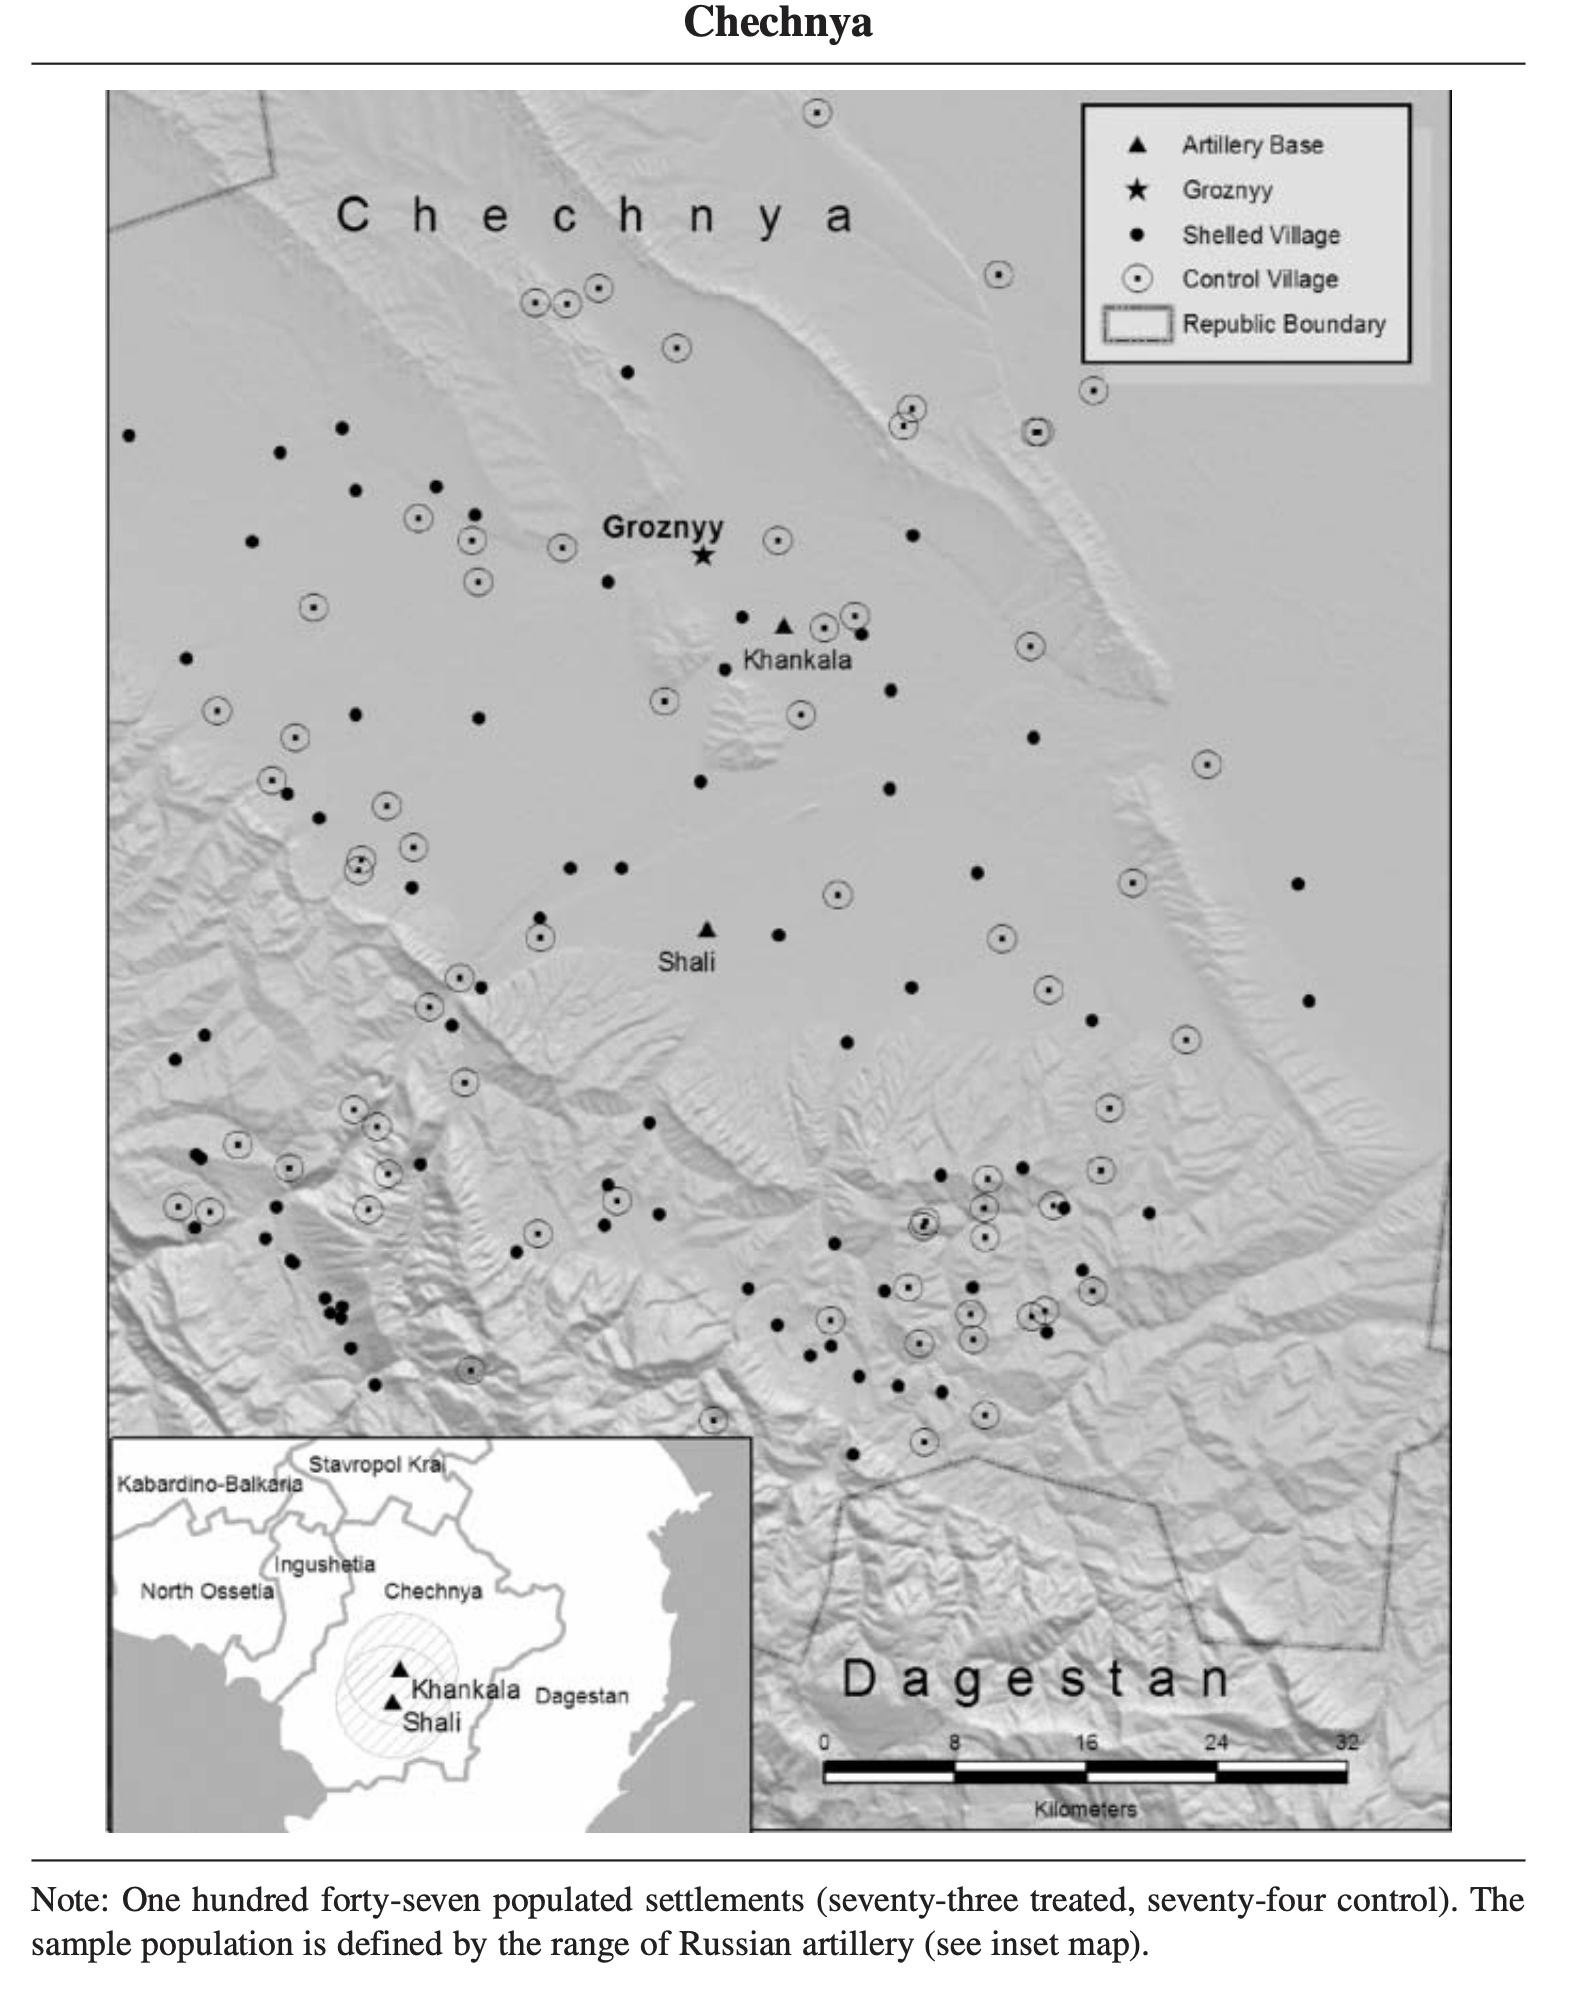
\includegraphics[width=0.9\textwidth,height=\textheight]{figs/lyall20092.png}
\end{frame}

\begin{frame}{}
\protect\hypertarget{section-4}{}
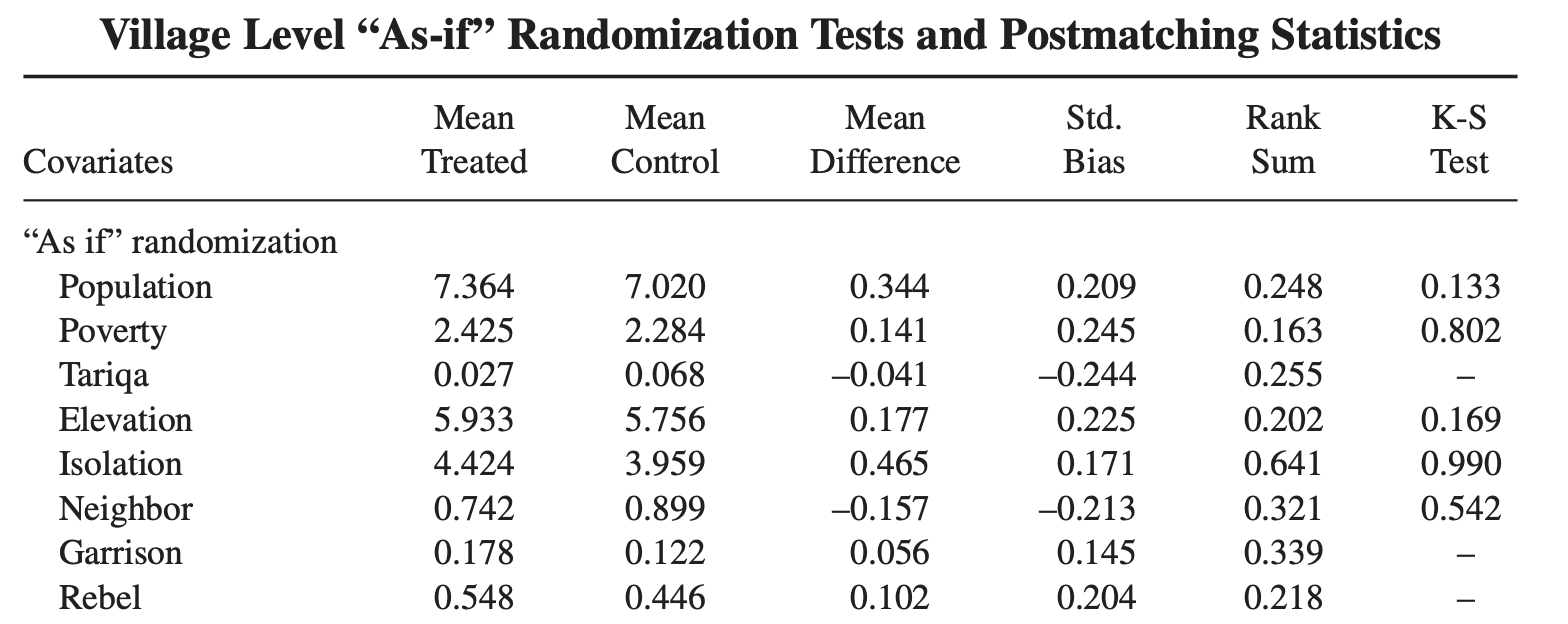
\includegraphics[width=0.9\textwidth,height=\textheight]{figs/lyall20093.png}
\end{frame}
<<<<<<< Updated upstream

\hypertarget{aleatorizaciuxf3n-de-la-asignaciuxf3n-al-tratamiento}{%
\section{Aleatorización de la asignación al
tratamiento}\label{aleatorizaciuxf3n-de-la-asignaciuxf3n-al-tratamiento}}
=======
>>>>>>> Stashed changes

\begin{frame}{Aleatorización de la asignación al tratamiento}
\protect\hypertarget{aleatorizaciuxf3n-de-la-asignaciuxf3n-al-tratamiento-1}{}
\begin{itemize}
\item
  Aleatorización significa que cada observación tiene una probabilidad
  conocida de asignación a las condiciones experimentales \emph{entre} 0
  y 1.
\item
  Ninguna unidad de la muestra experimental se asigna al tratamiento con
  certeza (probabilidad = 1) o al control con certeza (probabilidad =
  0).
\item
  Las unidades pueden variar en su probabilidad de asignación al
  tratamiento.
\item
  Por ejemplo, la probabilidad puede variar según el grupo: las mujeres
  pueden tener una probabilidad del 25\% de ser asignadas al
  tratamiento, mientras que los hombres tienen una probabilidad
  diferente.
\item
  Incluso puede variar entre individuos, aunque esto complicaría el
  análisis.
\end{itemize}
\end{frame}

\begin{frame}{Asignación aleatoria frente a muestreo aleatorio}
\protect\hypertarget{asignaciuxf3n-aleatoria-frente-a-muestreo-aleatorio}{}
\begin{itemize}
\item
  Aleatorización (del tratamiento): asignación de sujetos con
  probabilidad conocida a las condiciones experimentales.

  \begin{itemize}
  \item
    Esta asignación aleatoria del tratamiento puede combinarse con
    cualquier tipo de muestra (muestra aleatoria, muestra de
    conveniencia, etc.).
  \item
    Pero el tamaño y otras características de la muestra afectarán a la
    potencia y a la capacidad de extrapolar los resultados a otras
    poblaciones.
  \end{itemize}
\item
  Muestreo aleatorio (de la población): selección de los sujetos de la
  muestra a partir de una población con una probabilidad conocida.
\end{itemize}
\end{frame}

\begin{frame}{Aleatorización}
\protect\hypertarget{aleatorizaciuxf3n}{}
\begin{itemize}
\item
  Queremos la ATE, \(\overline{\tau_i}= \overline{Y_i(1)-Y_i(0)}\).
\item
  Haremos uso del hecho de que la media de las diferencias es igual a la
  diferencia de las medias:
\end{itemize}

\centering

ATE \(= \overline{Y_i(1)-Y_i(0)} = \overline{Y_i(1)}-\overline{Y_i(0)}\)
\end{frame}

\begin{frame}{Aleatorización}
\protect\hypertarget{aleatorizaciuxf3n-1}{}
\begin{itemize}
\item
  Asignamos \emph{aleatoriamente} algunas de nuestras unidades a la
  condición de tratamiento. Para estas unidades tratadas, medimos el
  resultado \(Y_i|T_i=1\), que es el mismo que \(Y_i(1)\) para estas
  unidades.
\item
  Como estas unidades se asignaron aleatoriamente al tratamiento, estos
  \(Y_i=Y_i(1)\) para las unidades tratadas representan el \(Y_i(1)\)
  para todas nuestras unidades.
\item
  En expectativa (o en promedio a través de experimentos repetidos
  (escrito \(E_R[]\))):
\end{itemize}

\centering

\(E_R[\overline{Y_i}|T_i=1]=\overline{Y_i(1)}\).

\begin{itemize}
\item
  El \(\overline{Y}|T_i=1\) es un estimador insesgado de la media
  poblacional de los resultados potenciales bajo tratamiento.
\item
  La misma lógica se aplica a las unidades asignadas aleatoriamente al
  control:
\end{itemize}

\centering

\(E_R[\overline{Y_i}|T_i=0]=\overline{Y_i(0)}\).
\end{frame}

\begin{frame}{Aleatorización}
\protect\hypertarget{aleatorizaciuxf3n-2}{}
\begin{itemize}
\tightlist
\item
  Así que podemos escribir un estimador para el ATE:
\end{itemize}

\centering

\(\hat{\overline{\tau_i}} = ( \overline{Y_i(1)} | T_i = 1 ) - ( \overline{Y_i(0)} | T_i = 0 )\)

\begin{itemize}
\tightlist
\item
  En la expectativa, o en promedio a través de experimentos repetidos,
  \(\hat{\overline{\tau_i}}\) es igual al ATE:
\end{itemize}

\centering

\(E_R[Y_i| T_i = 1 ] - E_R[Y_i | T_i = 0] = \overline{Y_i(1)} - \overline{Y_i(0)}\).

\begin{itemize}
\tightlist
\item
  Podemos simplemente tomar la diferencia de estos estimadores
  insesgados de \(\overline{Y_i(1)}\) y \(\overline{Y_i(0)}\) para
  obtener una estimación insesgada del ATE.
\end{itemize}
\end{frame}

\begin{frame}{Tres supuestos clave}
\protect\hypertarget{tres-supuestos-clave}{}
Para hacer afirmaciones causales con un experimento (o para juzgar si
nos creemos las afirmaciones de un estudio), necesitamos tres supuestos
fundamentales:

\begin{itemize}
\item
  Asignación aleatoria de los sujetos al tratamiento, lo que implica que
  recibir el tratamiento es estadísticamente independiente de los
  resultados potenciales de los sujetos.
\item
  Suposición estabilidad del valor del tratamiento unitario (SUTVA).
\item
  Excluibilidad, que significa que los resultados potenciales de un
  sujeto responden sólo al tratamiento definido, no a otros factores
  extraños que puedan estar correlacionados con el tratamiento.
\end{itemize}
\end{frame}

\begin{frame}{SUTVA, parte 1}
\protect\hypertarget{sutva-parte-1}{}
\begin{enumerate}
\item
  El resultado potencial de un sujeto sólo refleja si recibe o no el
  tratamiento. No se ve afectado por cómo se asignan los tratamientos a
  otros sujetos.

  \begin{itemize}
  \item
    Una violación clásica es el caso de las vacunas y sus efectos
    indirectos.
  \item
    Supongamos una persona en la condición de control (sin vacuna). Si
    su enfermedad (\(Y_i(0)\)) depende del estado de tratamiento de
    otras personas (si se vacunan o no), ¡es como si tuviera dos
    \(Y_i(0)\) diferentes!
  \item
    SUTVA (= stable unit treatment value assumption)
  \end{itemize}
\end{enumerate}
\end{frame}

\begin{frame}{SUTVA, parte 2}
\protect\hypertarget{sutva-parte-2}{}
\begin{enumerate}
\setcounter{enumi}{1}
\item
  No hay variaciones ocultas del tratamiento

  \begin{itemize}
  \item
    Digamos que el tratamiento es tomar una vacuna, pero hay dos tipos
    de vacunas y tienen ingredientes diferentes.
  \item
    Un ejemplo de violación es cuando la posibilidad de estar enfermo al
    recibir la vacuna (\(Y_i(1)\)) depende de la vacuna que haya tomado.
    Tendríamos dos \(Y_i(1)\) diferentes.
  \end{itemize}
\end{enumerate}
\end{frame}

\begin{frame}{Excluibilidad}
\protect\hypertarget{excluibilidad}{}
\begin{itemize}
\item
  La asignación del tratamiento no tiene ningún efecto sobre los
  resultados, excepto a través de su efecto sobre si se recibió el
  tratamiento.

  \begin{itemize}
  \item
    Es importante definir el tratamiento con precisión.
  \item
    También es importante mantener la simetría entre los grupos de
    tratamiento y de control (por ejemplo, mediante el enmascaramiento,
    con los mismos procedimientos de recogida de datos para todos los
    sujetos del estudio, etc.), de modo que la asignación al tratamiento
    sólo afecte al tratamiento recibido, y no a otras cosas como las
    interacciones con los investigadores que no se quieran definir como
    parte del tratamiento.
  \end{itemize}
\end{itemize}
\end{frame}

\begin{frame}{Aleatorización simple}
\protect\hypertarget{aleatorizaciuxf3n-simple}{}
\begin{itemize}
\item
  Para cada unidad, tiramos una moneda para ver si será tratada. Luego
  medimos la variable de resultado al mismo nivel que la moneda.
\item
  Las monedas no tienen que ser justas (50-50), pero debemos conocer la
  probabilidad de asignación al tratamiento.
\item
  No se puede garantizar un número concreto de unidades tratadas y
  unidades de control.
\item
  Ejemplo: Si tiene 6 unidades y lanza una moneda justa para cada una,
  tiene aproximadamente un 3\% de probabilidades de asignar
  \textbf{todas} las unidades al tratamiento o de asignar \textbf{todas}
  las unidades al control.
\end{itemize}
\end{frame}

\begin{frame}{Aleatorización completa}
\protect\hypertarget{aleatorizaciuxf3n-completa}{}
\begin{itemize}
\item
  Se asigna al tratamiento un número fijo \(m\) de \(N\) unidades.
\item
  La probabilidad de que una unidad se asigne al tratamiento es \(m/N\).
\item
  Es como tener una urna con \(N\) bolas, de las que \(m\) se marcan
  como tratamiento y \(N-m\) como control. Las loterías públicas
  utilizan este método.
\end{itemize}
\end{frame}

\end{document}
